\documentclass[titlepage]{article}
\usepackage[utf8]{inputenc}
\usepackage[english]{babel}
\usepackage{multirow}
\usepackage{float}
\usepackage{graphicx}
\usepackage{listings}
\usepackage{xcolor}
\usepackage{fancyhdr}
\usepackage{hyperref}
\usepackage{tabularx}
\newcolumntype{C}{>{\centering\arraybackslash}X}


\graphicspath{ {./img/} }

\pagestyle{fancy}
\fancyhf{}
\lhead{}
\chead{}
\rhead{\leftmark}
\lfoot{}
\cfoot{\thepage}
\rfoot{}
\renewcommand{\headrulewidth}{0pt}
\renewcommand{\lstlistingname}{Codice}

\DeclareFixedFont{\ttb}{T1}{txtt}{bx}{n}{9}
\DeclareFixedFont{\ttm}{T1}{txtt}{m}{n}{9}
\definecolor{deepblue}{rgb}{0,0,0.5}
\definecolor{deepred}{rgb}{0.6,0,0}
\definecolor{deepgreen}{rgb}{0,0.5,0}

\newcommand\pythonstyle{\lstset{
  language=Python,
  backgroundcolor=\color{white},
  basicstyle=\ttm,
  otherkeywords={self},
  keywordstyle=\ttb\color{deepblue},
  emph={MyClass,__init__},
  emphstyle=\ttb\color{deepred},
  stringstyle=\color{deepgreen},
  commentstyle=\color{red},
  frame=tb,
  showstringspaces=false,
  numbers=left,
  stepnumber=1,
  showstringspaces=false,
  tabsize=1,
  breaklines=true,
  breakatwhitespace=false,
}}

\lstnewenvironment{python}[1][]
{
\pythonstyle
\lstset{#1}
}
{}

\definecolor{mygreen}{rgb}{0,0.6,0}
\definecolor{mygray}{rgb}{0.5,0.5,0.5}
\definecolor{mymauve}{rgb}{0.58,0,0.82}
\definecolor{terminalbgcolor}{HTML}{330033}
\definecolor{terminalrulecolor}{HTML}{000099}
\newcommand{\lstconsolestyle}{
\lstset{
	backgroundcolor=\color{terminalbgcolor},
	basicstyle=\color{white}\fontfamily{fvm}\footnotesize\selectfont,
	breakatwhitespace=false,  
	breaklines=true,
	captionpos=b,
	commentstyle=\color{mygreen},
	deletekeywords={...},
	escapeinside={\%*}{*)},
	extendedchars=true,
	frame=single,
	keepspaces=true,
	keywordstyle=\color{blue},
	%language=none,
	morekeywords={*,...},
	numbers=none,
	numbersep=5pt,
  framerule=2pt,
	numberstyle=\color{mygray}\tiny\selectfont,
	rulecolor=\color{terminalrulecolor},
	showspaces=false,
	showstringspaces=false,
	showtabs=false,
	stepnumber=2,
	stringstyle=\color{mymauve},
	tabsize=2
}
}

\definecolor{delim}{RGB}{20,105,176}
\definecolor{numb}{RGB}{106, 109, 32}
\definecolor{string}{rgb}{0.64,0.08,0.08}

\lstdefinelanguage{json}{
    numbers=left,
    numberstyle=\small,
    frame=single,
    rulecolor=\color{black},
    showspaces=false,
    showtabs=false,
    breaklines=true,
    postbreak=\raisebox{0ex}[0ex][0ex]{\ensuremath{\color{gray}\hookrightarrow\space}},
    breakatwhitespace=true,
    basicstyle=\ttfamily\small,
    upquote=true,
    morestring=[b]",
    stringstyle=\color{string},
    literate=
     *{0}{{{\color{numb}0}}}{1}
      {1}{{{\color{numb}1}}}{1}
      {2}{{{\color{numb}2}}}{1}
      {3}{{{\color{numb}3}}}{1}
      {4}{{{\color{numb}4}}}{1}
      {5}{{{\color{numb}5}}}{1}
      {6}{{{\color{numb}6}}}{1}
      {7}{{{\color{numb}7}}}{1}
      {8}{{{\color{numb}8}}}{1}
      {9}{{{\color{numb}9}}}{1}
      {\{}{{{\color{delim}{\{}}}}{1}
      {\}}{{{\color{delim}{\}}}}}{1}
      {[}{{{\color{delim}{[}}}}{1}
      {]}{{{\color{delim}{]}}}}{1},
}

\lstdefinestyle{customc}{
  belowcaptionskip=1\baselineskip,
  breaklines=true,
  frame=L,
  xleftmargin=\parindent,
  language=C,
  showstringspaces=false,
  basicstyle=\footnotesize\ttfamily,
  keywordstyle=\bfseries\color{green!40!black},
  commentstyle=\itshape\color{purple!40!black},
  identifierstyle=\color{blue},
  stringstyle=\color{orange},
}

\lstdefinestyle{customasm}{
  belowcaptionskip=1\baselineskip,
  frame=L,
  xleftmargin=\parindent,
  language=[x86masm]Assembler,
  basicstyle=\footnotesize\ttfamily,
  commentstyle=\itshape\color{purple!40!black},
}

\title{Parallelization of random graph algorithms}
\author{Fabrizio Corriera}
\date{27/11/2023}

\begin{document}

\maketitle

\pagenumbering{roman}
\tableofcontents
\newpage
\pagenumbering{arabic}

\section{Introduction}
The scope of this work is to explore and analyse the parallelization of different random graph algorithms, using different techniques, and comparing the results.

Random graphs are mathematical models used to represent a wide range of complex systems, such as social networks, biological networks, and communication networks. They provide a way to study and understand the emergent properties of large, interconnected systems by introducing randomness into the structure of the graphs.

The general idea behind random graphs is to generate graphs with certain probabilistic properties, rather than specifying the connections between nodes explicitly. This randomness allows researchers to study the average behavior and characteristics of graphs within a certain probability distribution. Random graph models are particularly useful for capturing the inherent unpredictability and complexity of real-world networks.

Some common models and algorithms for generating random graphs include:

\begin{itemize}
    \item \textbf{Erdős-Rényi (ER) Model:} In the Erdős-Rényi model, edges are added between pairs of nodes with a fixed probability $p$. The resulting graphs often exhibit a phase transition, where below a certain probability, the graph is likely to consist of isolated components, and above that probability, a giant connected component emerges.
    \item \textbf{Watts-Strogatz Model:} The Watts-Strogatz model starts with a regular lattice and rewires edges with a certain probability. This small amount of randomness helps capture both the regularity found in some networks and the small-world phenomenon observed in many real-world networks.
    \item \textbf{Barabási-Albert  Model:} The Barabási-Albert model is a preferential attachment model where nodes are added to the graph one at a time. Each new node connects to existing nodes with a probability that is proportional to their degree. This model leads to scale-free networks, where a small number of nodes have a disproportionately large number of connections.
    \item \textbf{Random Geometric Graph (RGG):} A Random Geometric Graph (RGG) is a type of random graph where nodes are distributed randomly in a metric space, and edges are formed based on geometric proximity. In other words, nodes are points in a space, and an edge is established between two nodes if the distance between them is below a certain threshold. This model is particularly relevant in scenarios where the spatial arrangement of nodes plays a crucial role, such as wireless sensor networks, communication networks, or applications involving proximity-based interactions.
\end{itemize}

While random graph models offer valuable insights into the structural properties of networks, it is important to specify that they often fall short in fully capturing the complexity and nuanced characteristics of real-life networks, like heterogeneity, temporal dynamic, communities structure and many more.

Parallelization of this kind of algorithms is not a much discussed subject, nor it is considered a relevant matter when talking about parallelization. Some studies have been published mainly regarding the distributed version of these algorithms, but very few results may be found regarding local parallelization.

\section{Functional requirements}
The functional requirements for this project are:
\begin{itemize}
    \item Develop at least a functional parallelized version of a known random graph algorithm.
    \item Test the perfermance with different parameters with different orders of magnitude.
    \item Compare the performance of the linear version with the parallelized one.
\end{itemize}

The best result would be to be able to use different parallelization methods on different algorithms to truly be able to appreciate the differences in performance.

\section{Tools used}
For this work we have used the following tools:
\begin{itemize}
    \item \textbf{OpenCL:} OpenCL (Open Computing Language) is an open standard for parallel programming across heterogeneous platforms. It allows developers to write programs that can execute on various devices, including CPUs, GPUs, and accelerators, enabling efficient parallel processing for tasks like scientific simulations, image processing, and machine learning. OpenCL provides a framework for exploiting the computational power of diverse hardware architectures in a unified manner.
    \item \textbf{C programming language:} C, a general-purpose programming language, is widely used for its efficiency and versatility. OpenCL C is a subset of C designed for parallel programming within the OpenCL framework. Developers use the OpenCL API to create programs that leverage parallel computing across diverse devices, such as CPUs and GPUs, making it a powerful tool for high-performance computing and parallel processing tasks.
\end{itemize}

\section{OpenCL}
\subsection{A gentle introduction}
OpenCL, or Open Computing Language, is an open standard developed by the Khronos Group, designed to enable heterogeneous computing across various platforms. It provides a framework for parallel programming, allowing developers to harness the computational power of diverse devices, including CPUs, GPUs, and accelerators.

It introduces a parallel programming model where tasks are divided into work items, organized into work groups. These work items are executed concurrently, exploiting the parallel processing capabilities of the underlying hardware. OpenCL operates with a host-device model: the host, typically a CPU, manages the overall execution and launches tasks on the device, such as a GPU. The device executes the parallelized tasks specified by the OpenCL C language, that is a language tailored for parallel programming. It includes constructs for data parallelism, work item synchronization, and memory management specific to OpenCL.

OpenCL provides a hierarchical memory model, including global, local, and private memory spaces. Developers must carefully manage data movement between these spaces to optimize performance. OpenCL's execution model allows developers to specify how work items are divided into work groups, facilitating efficient parallel execution. This model is especially powerful for applications requiring massive parallelism, like image processing and scientific simulations.

The general steps for OpenCL workflow are:
\begin{enumerate}
    \item Platform and device discovery: we begin by discovering available OpenCL platforms and devices on a system. A platform represents a particular vendor's OpenCL implementation, while a device refers to a specific hardware unit, like a GPU or CPU.
    \item Kernel programming: we write OpenCL kernels, which are functions written in OpenCL C that define the behavior of a single work item. These kernels can be executed in parallel on multiple devices.
    \item Compilation and execution: OpenCL programs consist of both host code (typically written in C or another high-level language) and kernel code (written in OpenCL C). The host code manages the execution flow, while the kernel code is compiled and executed on the devices.
    \item Data transfer: efficient data transfer between the host and device is crucial. OpenCL provides functions to move data between the host and device memories, ensuring that the right data is available for computation.
    \item Synchronization and control: OpenCL provides mechanisms for synchronizing work items within a work group and controlling the overall execution flow. Events and barriers help manage dependencies and synchronization between different parts of the program.
\end{enumerate}

\subsection{Setting up an OpenCL program}
We will now illustrate technically the general steps needed to implement an OpenCL algorithm.

\begin{minipage}{\linewidth}
\begin{lstlisting}[language=C, style=customc, breaklines=true]
    //Configure the OpenCL environment
    cl_platform_id platform = 0;
    clGetPlatformIDs(1, &platform, NULL);
    cl_device_id device = 0;
    clGetDeviceIDs(platform, CL_DEVICE_TYPE_GPU, 1, &device, NULL);
    cl_context context = clCreateContext(NULL, 1, &device, NULL, NULL, NULL);
    cl_command_queue queue = clCreateCommandQueue(context, device, 0, NULL);
\end{lstlisting}
\end{minipage}

Here, in this example we first define and inizialize a variable of type \newline "cl\_platform\_id" and then use a function "clGetPlatformIDs" to assign it the value of the id of the first platform available. The function signature is:
\begin{itemize}
    \item clGetPlatformIDs(cl\_uint num\_entries, cl\_platform\_id *platforms, cl\_uint *num\_platforms)
    \begin{itemize}
        \item num\_entries: this parameter specifies the max number of entries we want to be appended to \textit{platforms}.
        \item platforms: this parameter specifies the variable where we want the IDs of the platforms to be appended. This variable will contain at most \textit{num\_entries} IDs or all the platforms available in the system, whichever is the minimum.
        \item num\_platforms: the function will return the total number of platforms available to this variable if specified.
    \end{itemize}
\end{itemize}

So, now we have the IDs for the platforms we want our kernel to be executed on. We now need to find the id of the devices. In order to do this, very similarly we define a  variable of type "cl\_device\_id" and then use a function "clGetDeviceIDs" to pass it the IDs for the desired devices. The function signature is:

\begin{itemize}
    \item clGetDeviceIDs(cl\_platform\_id platform, cl\_device\_type device\_type,\newline cl\_uint num\_entries, cl\_device\_id *devices, cl\_uint *num\_devices)
    \begin{itemize}
        \item platform: we pass to the function the ID of the platform we are querying for devices.
        \item device\_type: a bitfield that identifies the type of OpenCL device. The \textit{device\_type} can be used to query specific OpenCL devices or all OpenCL devices available.
        \item num\_entries: this parameter specifies the max number of entries we want to be appended to \textit{devices}.
        \item devices: this parameter specifies the variable where we want the IDs of the devices to be appended. This variable will contain at most \textit{num\_entries} IDs or all the devices whose type matches \textit{device\_type}, whichever is the minimum.
        \item num\_devices: the function will return the total number of devices available to this variable if specified.
    \end{itemize}
\end{itemize}

Now we are ready to define our context. An OpenCL context is created with one or more devices. Contexts are used by the OpenCL runtime for managing objects such as command-queues, memory, program and kernel objects and for executing kernels on one or more devices specified in the context. To define the context we use the "clCreateContext" function:

\begin{itemize}
    \item clCreateContext(cl\_context\_properties *properties, cl\_uint num\_devices, const cl\_device\_id *devices, void *pfn\_notify(const char *errinfo, const void *private\_info, size\_t cb, void *user\_data), void *user\_data, cl\_int *errcode\_ret)
    \begin{itemize}
        \item properties: specifies a list of context property names and their corresponding values.\textit{properties} can be NULL in which case the platform that is selected is implementation-defined.
        \item num\_devices: this variable contains the number of devices specified in \textit{devices}.
        \item devices: a pointer to a list of unique devices returned by \textit{clGetDeviceIDs} for a platform.
        \item pfn\_notify: a callback function that can be registered by the application. This callback function will be used by the OpenCL implementation to report information on errors that occur in this context.
        \item user\_data: passed as the \textit{user\_data} argument when \textit{pfn\_notify} is called. \textit{user\_data} can be NULL.
        \item errcode\_ret: returns an appropriate error code. If \textit{errcode\_ret} is NULL, no error code is returned. 
    \end{itemize}
\end{itemize}

After defining the context we have to define a command queue. An OpenCL command queue is used by the host application to send kernels and data transfer functions to a device for execution. By enqueueing commands into a command queue, kernels and data transfer functions may execute asynchronously and in parallel with application host code. We use the "clCreateCommandQueue" function in order to do this.

\begin{itemize}
    \item clCreateCommandQueue(cl\_context context, cl\_device\_id device, \newline cl\_command\_queue\_properties properties, cl\_int *errcode\_ret)
    \begin{itemize}
        \item context: we must pass an OpenCL context in order to create a command queue.
        \item device: must be a device associated with \textit{context}.
        \item properties: specifies a list of properties for the command-queue.
        \item errcode\_ret: returns an appropriate error code. If \textit{errcode\_ret} is NULL, no error code is returned. 
    \end{itemize}
\end{itemize}

After the configuration of our OpenCL context, we can go on and talk about compiling the kernel.

\begin{minipage}{\linewidth}
\begin{lstlisting}[language=C, style=customc, breaklines=true]
    //Compile the kernel
    cl_program program = clCreateProgramWithSource(context, 1, &kernelstring, NULL, NULL);
    clBuildProgram(program, 0, NULL, "", NULL, NULL);
\end{lstlisting}
\end{minipage}

This is one of the main features that highlights the flexibility of OpenCL. What we are doing with these lines of code is dinamically compiling code (that can either be defined as a string in the same file containing the main function or can be written in another file).

The function \textit{clCreateProgramWithSource} creates a program object for a context, and loads the source code specified by the text strings in the strings array into the program object. 

\begin{itemize}
    \item clCreateProgramWithSource(cl\_context context, cl\_uint count, const char **strings, const size\_t *lengths, cl\_int *errcode\_ret)
    \begin{itemize}
        \item context: the OpenCL context on which we want to run the program.
        \item count: this parameter specifies the number of pointers contained in \textit{strings}.
        \item strings: an array of pointers to optionally null-terminated character strings that make up the source code.
        \item  lengths: an array with the number of chars in each string (the string length). If an element in \textit{lengths} is zero, its accompanying string is null-terminated. If \textit{lengths} is NULL, all strings in the \textit{strings} argument are considered null-terminated. Any length value passed in that is greater than zero excludes the null terminator in its count.
        \item errcode\_ret: returns an appropriate error code. If \textit{errcode\_ret} is NULL, no error code is returned.
    \end{itemize}
\end{itemize}

The clBuildProgram instead builds (compiles and links) a program executable from the program source or binary.

\begin{itemize}
    \item clBuildProgram(cl\_program program, cl\_uint num\_devices, const cl\_device\_id *device\_list, const char *options, void (CL\_CALLBACK *pfn\_notify)(cl\_program program, void *user\_data), void *user\_data)
    \begin{itemize}
        \item program: the variable containing the program object.
        \item num\_devices: The number of devices listed in \textit{device\_list}.
        \item device\_list: a pointer to a list of devices associated with program. If \textit{device\_list} is a NULL value, the program executable is built for all devices associated with \textit{program} for which a source or binary has been loaded.
        \item options: a pointer to a null-terminated string of characters that describes the build options to be used for building the program executable.
        \item pfn\_notify: a function pointer to a notification routine. The notification routine is a callback function that an application can register and which will be called when the program executable has been built (successfully or unsuccessfully). If \textit{pfn\_notify} is not NULL, clBuildProgram does not need to wait for the build to complete and can return immediately once the build operation can begin.
        \item user\_data: passed as an argument when \textit{pfn\_notify} is called. \textit{user\_data} can be NULL.
    \end{itemize}
\end{itemize}

\begin{minipage}{\linewidth}
\begin{lstlisting}[language=C, style=customc, breaklines=true]
    //Configure the kernel
    cl_kernel kernel = clCreateKernel(program, "ER", NULL);
\end{lstlisting}
\end{minipage}

This function creates a kernel object, that is basically a function declared in a program.

\begin{itemize}
    \item cl\_kernel clCreateKernel(cl\_program program, const char *kernel\_name, cl\_int *errcode\_ret)
    \begin{itemize}
        \item program: a program object with a successfully built executable.
        \item kernel\_name: a function name in the program declared with the \_\_kernel qualifier.
        \item errorcode\_ret: returns an appropriate error code. If \textit{errcode\_ret} is NULL, no error code is returned.
    \end{itemize}
\end{itemize}

\subsection{Memory management}

Before executing the program we just built we should make some considerations regarding the memory: the program we built will not run on the same device on which we are executing the host code, so it will not be able to access the memory registers where we instancieted the variables declared on the host program. Therefore it is necessary to copy the variables needed for the program execution on the device memory.

\begin{minipage}{\linewidth}
\begin{lstlisting}[language=C, style=customc, breaklines=true]
    //Prepare OpenCL memory objects
    cl_mem bufG = clCreateBuffer(context, CL_MEM_READ_WRITE,
        N*N*sizeof(int), NULL, NULL);
\end{lstlisting}
\end{minipage}

clCreateBuffer, as its name suggestes, creates a buffer object.

\begin{itemize}
    \item clCreateBuffer(cl\_context context, cl\_mem\_flags flags, size\_t size, void \newline *host\_ptr, cl\_int *errcode\_ret)
    \begin{itemize}
        \item context: a valid OpenCL context used to create the buffer object.
        \item flags: a bit-field that is used to specify allocation and usage information such as the memory arena that should be used to allocate the buffer object and how it will be used.
        \item size: the size in bytes of the buffer memory object to be allocated.
        \item host\_ptr: a pointer to the buffer data that may already be allocated by the application.
        \item errcode\_ret: returns an appropriate error code. If \textit{errcode\_ret} is NULL, no error code is returned.
    \end{itemize}
\end{itemize}

\begin{minipage}{\linewidth}
\begin{lstlisting}[language=C, style=customc, breaklines=true]
    //Copy the data to the device
    clEnqueueWriteBuffer(queue, bufG, CL_TRUE, 0,
        N*N*sizeof(int), G, 0, NULL, NULL);
\end{lstlisting}
\end{minipage}

After allocating the memory we must copy the data in the buffer.

\begin{itemize}
    \item clEnqueueWriteBuffer(cl\_command\_queue command\_queue, cl\_mem buffer, cl\_bool blocking\_write, size\_t offset, size\_t size, const void *ptr, cl\_uint num\_events\_in\_wait\_list, const cl\_event *event\_wait\_list, cl\_event *event)
    \begin{itemize}
        \item command\_queue: is a valid host command-queue in which the write command will be queued. \textit{command\_queue} and buffer must be created with the same OpenCL \textit{context}.
        \item buffer: the buffer object we are writing on.
        \item blocking\_write: indicates if the write operations are blocking (CL\_TRUE) or nonblocking(CL\_FALSE).
        \item offset: the offset in bytes in the buffer object to write to.
        \item size: the size in bytes of data being written.
        \item ptr: the pointer to buffer in host memory where data is to be written from.
        \item num\_events\_in\_wait\_list: this parameter specifies the size of the array \textit{event\_wait\_list}. If \textit{event\_wait\_list} is NULL, \textit{num\_events\_in\_wait\_list} must be 0. 
        \item event\_wait\_list: this parameter specifies events that need to complete before this particular command can be executed. If it is NULL, then this particular command does not wait on any event to complete.
        \item event: returns an event object that identifies this particular write command and can be used to query or queue a wait for this particular command to complete. \textit{event} can be NULL in which case it will not be possible for the application to query the status of this command or queue a wait for this command to complete.
    \end{itemize}
\end{itemize}

\begin{minipage}{\linewidth}
\begin{lstlisting}[language=C, style=customc, breaklines=true]
    //Set kernel arguments
    clSetKernelArg(kernel, 0, sizeof(unsigned int), (void*)&N);
    clSetKernelArg(kernel, 1, sizeof(double), (void*)&p);
    clSetKernelArg(kernel, 2, sizeof(unsigned int), (void*)&seed);
    clSetKernelArg(kernel, 3, sizeof(unsigned int), (void*)&base);
    clSetKernelArg(kernel, 4, sizeof(cl_mem), (void*)&bufG);
\end{lstlisting}
\end{minipage}

After we create the kernel and before we run it we must pass it its arguments, in the same order we defined in the \_\_kernel program function.

\begin{itemize}
    \item cl\_int clSetKernelArg(cl\_kernel kernel, cl\_uint arg\_index, size\_t arg\_size, const void *arg\_value)
    \begin{itemize}
        \item kernel: a valid kernel object.
        \item arg\_index: the index of the argument we are passing to the kernel. Arguments to the kernel are referred by indices that go from $0$ for the leftmost argument to $n - 1$, where $n$ is the total number of arguments declared by a kernel.
        \item arg\_size: the size of the argument value. If the argument is a memory object, the size is the size of the memory object. 
        \item arg\_value: the pointer to data that should be used as the argument value for argument specified by \textit{arg\_index}. The argument data pointed to by \textit{arg\_value} is copied and the \textit{arg\_value} pointer can therefore be reused by the application after clSetKernelArg returns. The argument value specified is the value used by all API calls that enqueue \textit{kernel} (clEnqueueNDRangeKernel) until the argument value is changed by a call to clSetKernelArg for \textit{kernel}.
    \end{itemize}
\end{itemize}

\begin{minipage}{\linewidth}
\begin{lstlisting}[language=C, style=customc, breaklines=true]
    // Copy the output back to CPU memory
    clEnqueueReadBuffer(queue, bufG, CL_TRUE, 0, N*N*sizeof(int),
        G, 0, NULL, NULL);
\end{lstlisting}
\end{minipage}

As we can write on a buffer we can also read from it.

\begin{itemize}
    \item clEnqueueReadBuffer(cl\_command\_queue command\_queue, cl\_mem buffer, cl\_bool blocking\_read, size\_t offset, size\_t size, const void *ptr, cl\_uint num\_events\_in\_wait\_list, const cl\_event *event\_wait\_list, cl\_event *event)
    \begin{itemize}
        \item command\_queue: is a valid host command-queue in which the write command will be queued. \textit{command\_queue} and buffer must be created with the same OpenCL \textit{context}.
        \item buffer: the buffer object we are writing on.
        \item blocking\_read: indicates if the read operations are blocking (CL\_TRUE) or nonblocking(CL\_FALSE).
        \item offset: the offset in bytes in the buffer object to write to.
        \item size: the size in bytes of data being read.
        \item ptr: the pointer to buffer in host memory where data is to be read into.
        \item num\_events\_in\_wait\_list: this parameter specifies the size of the array \textit{event\_wait\_list}. If \textit{event\_wait\_list} is NULL, \textit{num\_events\_in\_wait\_list} must be 0. 
        \item event\_wait\_list: this parameter specifies events that need to complete before this particular command can be executed. If it is NULL, then this particular command does not wait on any event to complete.
        \item event: returns an event object that identifies this particular write command and can be used to query or queue a wait for this particular command to complete. \textit{event} can be NULL in which case it will not be possible for the application to query the status of this command or queue a wait for this command to complete.
    \end{itemize}
\end{itemize}

\subsection{Executing the kernel}
\begin{minipage}{\linewidth}
\begin{lstlisting}[language=C, style=customc, breaklines=true]
        // Run the kernel
        const size_t local[2] = { TS, TS };
        const size_t global[2] = { N, N };
        clEnqueueNDRangeKernel(queue, kernel, 2, NULL, global, local, 0, NULL, &event);

        // Wait for calculations to be finished
        clWaitForEvents(1, &event);
\end{lstlisting}
\end{minipage}

The main function of this snippet of code is clEnqueueNDRangeKernel, that, as the name suggests, enqueues a command to execute a kernel on a device.

\begin{itemize}
    \item clEnqueueNDRangeKernel(cl\_command\_queue command\_queue, cl\_kernel kernel, cl\_uint work\_dim, const size\_t *global\_work\_offset, const size\_t *global\_work\_size, const size\_t *local\_work\_size, cl\_uint num\_events\_in\_wait\_list, const cl\_event *event\_wait\_list, cl\_event *event)
    \begin{itemize}
        \item command\_queue: a valid command-queue. The kernel will be queued for execution on the device associated with \textit{command\_queue}.
        \item kernel: a valid kernel object. The OpenCL context associated with \textit{kernel} and \textit{command\_queue} must be the same.
        \item work\_dim: the number of dimensions used to specify the global work-items and work-items in the work-group. \textit{work\_dim} must be greater than zero and less than or equal to three.
        \item global\_work\_offset: this parameter can be used to specify an array of \textit{work\_dim} unsigned values that describe the offset used to calculate the global ID of a work-item instead of having the global IDs always start at offset (0, 0,... 0). In the version of OpenCL we used (1.0) it must be set to NULL.
        \item global\_work\_size: this parameter is a pointer to an array of \textit{work\_dim} unsigned values that describe the number of global work-items in \textit{work\_dim} dimensions that will execute the kernel function. The total number of global work-items is computed as the product of all the elements of the array pointed by \textit{global\_work\_size}
        \item local\_work\_size: this parameter is a pointer to an array of \textit{work\_dim} unsigned values that describe the number of work-items that make up a work-group (also referred to as the size of the work-group) that will execute the kernel specified by \textit{kernel}. The total number of work-items in the work-group must be less than or equal to the CL\_DEVICE\_MAX\_WORK\_GROUP\_SIZE value specified in table of OpenCL Device Queries for clGetDeviceInfo. \textit{local\_work\_size} can also be a NULL value in which case the OpenCL implementation will determine how to be break the global work-items into appropriate work-group instances.
        \item num\_events\_in\_wait\_list: specify the size of the array pointed by \textit{event\_wait\_list}.
        \item event\_wait\_list: specify events that need to complete before this particular command can be executed. If \textit{event\_wait\_list} is NULL, then this particular command does not wait on any event to complete.
        \item event: returns an event object that identifies this particular kernel execution instance. Event objects are unique and can be used to identify a particular kernel execution instance later on. If \textit{event} is NULL, no event will be created for this kernel execution instance.
    \end{itemize}
\end{itemize}

\section{Development}
We will now analyse and understand how the random graph algorithms we briefly described earlier can be parallelized.
\subsection{Erdős-Rényi Model}
The Erdős-Rényi model, as we said earlier is a totally random model, so the only parameters in this model are:
\begin{itemize}
    \item $N$ = the number of nodes in the graph.
    \item $p$ = the probability that two nodes will form an edge between them.
\end{itemize}

\begin{minipage}{\linewidth}
\begin{lstlisting}[language=C, style=customc, breaklines=true]
#define DIM 100

#define P 0.3

#define SEED 349872935

int main(int argc, char *argv[]) {
    unsigned int N = DIM; // Number of nodes
    double p = P; // Probability of edge creation
    double r; // Random number
    int i, j; // Iterators
    int* graph = (int*)malloc(N*N*sizeof(int*));
    clock_t start, end;
    double cpu_time_used;

    // Set the random seed
    srand(SEED);
\end{lstlisting}
\end{minipage}

The variable "graph" as we can see is an array of int that has length of $N^2$. So we are using an adjacency matrix to represent our graph, and we decided  to use an array instead of a matrix because of the explicit memory allocation, that gives us more control on how the memory is used.

The algorithm then just iterates through every node couple (so we have a for loop that iterates $N^2$ times), sample a random number, checks if that random number is lower than the threshold we declared, and if it the case than an edge is created between the two nodes.

\begin{minipage}{\linewidth}
\begin{lstlisting}[language=C, style=customc, breaklines=true]
for (i = 0; i < N; i++) {
    for (j = 0; j < N; j++) {
        if (i == j) {
            graph[i*N+j] = 0;  // No self-loops
        }
        else {
            // Generate a random number between 0 and 1
            r = (double)rand() / RAND_MAX;
            // Check if an edge should be created
            graph[i*N+j] = (r < p) ? 1 : 0;
        }
    }
}
\end{lstlisting}
\end{minipage}

As we can see, the general idea of the algorithm is very simple. Here we are showing the implementation for a directed graph; if we would have liked to have an implementation for an undirected graph, the only difference would have been to se the value to 1 not only to the position $(i,j)$, but to the position $(j,i)$ as well.

It is easy to see that the whole for loop is highly parallelizable, and since we don't have any read access to the memory and we must do $N^2$ write operations in any case, we can easily manage this problem as a 2-D problem with $N^2$ threads (one for each couple of nodes).

We then proceed writing the following kernel code for OpenCL:

\begin{minipage}{\linewidth}
\begin{lstlisting}[language=C, style=customc, breaklines=true]
const char *kernelstring =
    "__kernel void ER(const unsigned int N, const double p, const uint seed, const uint base,"
    "                 __global int* G){"
    "   const int globalNode_i = get_global_id(0);"
    "   const int globalNode_j = get_global_id(1);"
    "   uint seed_x = (seed + globalNode_i + globalNode_j) * (globalNode_i + 1) << globalNode_i;"
    "   uint t = seed_x ^ (seed_x << 11);"
    "   uint result = base ^ (base >> 19) ^ (t ^ (t >> 8));"
    "   double rand = (double) (result%56891279) / 56891279;"
    "   if ((rand<p) && (globalNode_i!=globalNode_j)){"
    "       G[globalNode_i*N+globalNode_j] = 1;"
    "   }"
    "   else G[globalNode_i*N+globalNode_j] = 0;"
    "}";
\end{lstlisting}
\end{minipage}

As we said earlier we can define the kernel code as a string, but it has the same structure as any other function declared in C. We can see the modifier \textit{\_\_kernel} written before the type of the function (void) and then the name of the function.

The arguments for the kernel are:
\begin{enumerate}
    \item N: the number of nodes of the graph.
    \item p: the probability to create a new edge.
    \item seed and base: these two values are necessary in order to create a working rng in OpenCL, since, at the best of our knowledge there is no random number generator defined natively in OpenCL C language.
    \item G: this parameter with the \textit{\_\_global} modifier is the buffer we declared earlier in the host code, that refers to the adjacency matrix.
\end{enumerate}

The first thing we do is to call the \textit{get\_global\_id} function, specifying the dimension we are refering to (0 or 1 in this case since we are working with a 2-D problem). The two numbers we get, \textit{globalNode\_i} and \textit{globalNode\_j} will both be the identifiers of the work-group we are currently in and the indices of the nodes (just like i and j in the for loop we saw int the sequential algorithm).

We then proceed to obtain our random number, using a version we defined of the xorshift algorithm.

\begin{minipage}{\linewidth}
\begin{lstlisting}[language=C, style=customc, breaklines=true]
uint seed_x = (seed + globalNode_i + globalNode_j) *
    (globalNode_i + 1) << globalNode_i;
uint t = seed_x ^ (seed_x << 11);
uint result = base ^ (base >> 19) ^ (t ^ (t >> 8));
double rand = (double) (result%56891279) / 56891279;
\end{lstlisting}
\end{minipage}

In each workgroup we must make sure to obtain a different random number, and that's why we modify the seed using the global IDs. We then proceed to do some hash operations using xor and shifts, enough to obtain a number from which we cannot obtain the original seed and base. We then cast the random int we obtained to double, do a module operation for a user defined number, and divide by that same number. This way we will obtain a number in range $[0,1[$.

In the end, exactly like the sequential ER algorithm, we compare the random number with our probability value, and if it's the lesser number, we will create the edge, otherwise we will not.

\begin{minipage}{\linewidth}
\begin{lstlisting}[language=C, style=customc, breaklines=true]
if ((rand<p) && (globalNode_i!=globalNode_j)){
    G[globalNode_i*N+globalNode_j] = 1;
}
else G[globalNode_i*N+globalNode_j] = 0;
\end{lstlisting}
\end{minipage}

It is important to specify that we decided to implement the ER random graph algorithm for a directed graph, instead of an undirected one (which is the most common version), because it is more efficient to parallelize. In an undirected ER random graph generator, we would not need $N^2$ loops to complete the algorithm, because this way we would explore each couple of nodes exactly two times. Below would be the most efficient way to implement the sequential algorithm for ER random graph generation.

\begin{minipage}{\linewidth}
\begin{lstlisting}[language=C, style=customc, breaklines=true]
for (i = 0; i < N; i++) {
    for (j = i+1; j < N; j++) {
        // Generate a random number between 0 and 1
        double r = (double)rand() / RAND_MAX;
        // Check if an edge should be created
        graph[i][j] = (r < PROB) ? 1 : 0;
        graph[j][i] = graph[i][j]; // Undirected graph, so mirror the edge
    }
}
\end{lstlisting}
\end{minipage}

It is not possible to parallelize efficiently this kind of behavior with an OpenCL kernel.

\subsection{Watts-Strogatz Model}
The Watts-Strogatz model, similarly to the ER model we need to generate a random number that will shape the randomness of the graph. In this model, however, we start with a given structure, that is a ring lattice, that we reshape randomly.

The parameters we need for this algorithm are:
\begin{itemize}
    \item $N$ = the number of nodes in the graph.
    \item $p$ = the probability that an edge will be rewired.
    \item $k$ = the initial number of edges for each node.
\end{itemize}

\begin{minipage}{\linewidth}
\begin{lstlisting}[language=C, style=customc, breaklines=true]
#define DIM 100

#define P 0.3

#define INIT_CONN 4

#define SEED 349872935

int main() {
    unsigned int N = DIM;          // Number of nodes
    double PROB = P;    // Probability of edge creation
    int K = INIT_CONN;
    double r;
    int i, j, l;
    int* G = (int*)malloc(N*N*sizeof(int*));
    clock_t start, end;
    double cpu_time_used;

    // Set the random seed
    srand(SEED);
\end{lstlisting}
\end{minipage}

One important detail to keep in mind is that $k$ must always be an even number, because each node $n$ must have the same number of edges with its $n+i\pmod{N}$ neighbors and its $n-i\pmod{N}$ neighbors, $\forall i \in [1, k/2]$.

And so, the algorithm is written this way:

\begin{minipage}{\linewidth}
\begin{lstlisting}[language=C, style=customc, breaklines=true]
for (i=0; i<N*N; i++) { G[i] = 0; }
for (i = 0; i < N; i++) {
    for (j = 1; j <= K/2; j++){
        r = (double)rand() / RAND_MAX;
        if (r<PROB) {
            do{
                l = (rand() % (N-K-2)) + (K/2) + 1;
            } while (G[i*N+((i+l)%N)] == 1);
            G[i*N+((i+l)%N)] = 1;
            G[((i+l)%N)*N+i] = 1;
        }
        else {
            G[i*N+((i+j)%N)] = 1;
            G[((i+j)%N)*N+i] = 1;
        }
    }
}
\end{lstlisting}
\end{minipage}

Basically, after initializing the whole adjacency matrix to $0$, we loop through the nodes, and for every node in the graph we explore its next $k/2$ neighbors, and, based on the result of the rng we decide if we will create a shortcircuit in the graph or if we will connect the two nodes like we are expected to.

This apporach is sligthly more efficient than the one where we first create the lattice ring and then proceed to check for the generation of shortcircuits, but the result is identical, since, if we were to set $p=1$ we would still get a lattice ring.

The computation complexity for this algorithm is not deterministic because of its random nature: once we are in the case where we have to create a shortcircuit we must select a new random node for the new edge, and doing so we can't connect two already connected edges; that's why we use a do-while loop to choose the node to which we will connect and that can take a variable amount of time. For this reason we wrote also a modified version of the algorithm were in the end the number of edges will not be exactly $N*(k/2)$ but it will be $|e|\le N*(k/2)$.

\begin{minipage}{\linewidth}
\begin{lstlisting}[language=C, style=customc, breaklines=true]
for (i=0; i<N*N; i++) { G[i] = 0; }
for (i = 0; i < N; i++) {
    for (j = 1; j <= K/2; j++){
        r = (double)rand() / RAND_MAX;
        if (r<PROB) {
            l = (rand() % (N-K-2)) + (K/2) + 1;
            G[i*N+((i+l)%N)] = 1;
            G[((i+l)%N)*N+i] = 1;
        }
        else {
            G[i*N+((i+j)%N)] = 1;
            G[((i+j)%N)*N+i] = 1;
        }
    }
}
\end{lstlisting}
\end{minipage}

And our parallelized version of the algorithm will be based on this one, in order to avoid concurrential accesses to the memory. At first sight, this seems like a 2-D problem, like the ER one, but actually, we can parallelize it in a 1-D way, having $N$ workgroups instead of $N^2$, and then loop inside them for $k/2$ times, reducing sensibly the computation time.

\begin{minipage}{\linewidth}
\begin{lstlisting}[language=C, style=customc, breaklines=true]
const char *kernelstring =
    "__kernel void WS(const unsigned int N, const double p, const int k, const uint seed, const uint base,"
    "   __global int* G){"
    "   const int globalNode = get_global_id(0);"
    "   for (int i = 1; i <= k/2; i++){"
    "       uint seed_x = (seed + globalNode + i) * (globalNode + 1) << globalNode;"
    "       uint t = seed_x ^ (seed_x << 11);"
    "       uint result = base ^ (base >> 19) ^ (t ^ (t >> 8));"
    "       double rand = (double) (result%56891279) / 56891279;"
    "       if ((rand<p)){"
    "           uint seed_x = (seed + globalNode + i) * (globalNode + 1) << globalNode;"
    "           uint t = seed_x ^ (seed_x << 11);"
    "           uint result = base ^ (base >> 19) ^ (t ^ (t >> 8));"
    "           int rand = (result%(N-k-2)) + (k/2) + 1;"
    "           G[globalNode*N+((globalNode+rand)%N)] = 1;"
    "           G[((globalNode+rand)%N)*N+globalNode] = 1;"
    "       }"
    "       else {"
    "           G[globalNode*N+((globalNode+i)%N)] = 1;"
    "           G[((globalNode+i)%N)*N+globalNode] = 1;"
    "       }"
    "   }"
    "}";
\end{lstlisting}
\end{minipage}

As we can see in this kernel we call the \textit{get\_global\_id} function just one time, because the problem is a 1-D problem. In the kernel we use a for loop to iterate through the $k/2$ connections. Again here we use the xorshift algorithm for the rng, and we must use it a first time for the probability to create a shortcircuit, and a second time to find a new node to connect to.

\subsection{Barabási-Albert Model}
The BA model is once more a model that has a probabilistic behaviour, but it does not rely on a uniform distribution statistically speaking, so the approach is a bit more complicated. Each node will prefer to connect to the nodes in the network that already are well connected, and this is a behaviour commonly saw in the real life networks.

The parameters for the BA algorithm are:
\begin{itemize}
    \item $N$: the number of nodes of the graph.
    \item $M$: the number of edges that each node will have when added to the graph.
\end{itemize}

From parameter $M$ we also obtain the starting number of nodes in the graph ($M_0>M$).

\begin{minipage}{\linewidth}
\begin{lstlisting}[language=C, style=customc, breaklines=true]
#define DIM 100

#define M 2

#define SEED 349872935

#define BASE 569872384

#define TS 10 // Threadblock sizes

int main(int argc, char *argv[]) {
    int i, j, k, m, a, r;
    unsigned int N = DIM; // Number of nodes
    int* deg = (int*)malloc(N*sizeof(int*)); // Array with the degrees of the nodes
    int* graph = (int*)malloc(N*N*sizeof(int*));
    unsigned int edges; // We just need the number of edges because we know that the sum of the degrees
    //in an undirected graph is 2|E|
    clock_t start, end;
    double cpu_time_used;

    // Set the random seed
    srand(SEED);
\end{lstlisting}
\end{minipage}

As we can see we need some additional variables to implement this algorithm:
\begin{itemize}
    \item deg: this is an array of size $N$ where we store the degree score of every node in the graph (the degree is the number of edges it is connected to).
    \item edges: this value stores the total number of edges in the network and this value is extremely important because in an undirected graph, the total degree of the network is $D_{Tot}=2|E|$. And we need the total degree of the graph in order to compute the probabilities  for the connection to a certain node, that, in literature is defined as $p_i=\frac{k_i}{\sum_j k_j}$, where $k$ is the degree of the node.
\end{itemize}

\begin{minipage}{\linewidth}
\begin{lstlisting}[language=C, style=customc, breaklines=true]
for (i=0; i<N; i++) { deg[i] = 0; } // Initialize the degree array
for (i=0; i<N*N; i++) { graph[i] = 0; } // Initialize the matrix
edges = 0;
        
// Set the starting M+1 nodes with M starting edges
for (i = 1; i <= M; i++){
    graph[i] = 1;
    graph[i*N] = 1;
    deg[i] += 1;
    edges += 1;
}
deg[0] = M;
\end{lstlisting}
\end{minipage}

In the first phase of the algorithm we have $n>M$ nodes, specifically in our implementation we have $M+1$ nodes, with $M$ connections. As default we connect all the $M$ nodes after the node $0$ to said node $0$, creating this way the first hub, and preferential attachment, of the graph.

After this first step we implemented the algorithm this way:

\begin{minipage}{\linewidth}
\begin{lstlisting}[language=C, style=customc, breaklines=true]
for (i = M+1; i < N; i++) { // For every node
    m = 0;
    while (deg[i] < M) { // For M times
        r = rand()%(edges*2); // We find our random value in a natural range of numbers instead of
        //[0,1]. This way we will need much less operations
        for (j = 0; j<N; j++) { // For every node we can connect to
            a = 0; // Initialize our probability
            for (k = 0; k<=j; k++) {
                a += deg[k]; //Compute the probability
            }
            if (r < a) {
                if (graph[i*N+j] == 0 ){
                    graph[i*N+j] = 1;
                    graph[j*N+i] = 1;
                    deg[i] += 1;
                    deg[j] += 1;
                    edges += 1;
                    m += 1;
                    break;
                }
            }
        }
    }
}
\end{lstlisting}
\end{minipage}

This algorithm requires us to update the probabilities to connect to a certain node after the creation of each edge; that's why for each node we must do $M$ loops and inside each one of them we need to do $N$ more loops to compute the new probability distribution.

As we can see, instead of generating a random number in range $[0,1[$, we create a random number in range $[0,2|E|[$, and we also compute the probability without normalizing it. This way we can avoid 2 floating point operations that would be executed every iteration of the inner loop structure.

Analyzing this algorithm it is easy to notice how it is an algorithm that is intrinsically sequential, because every edge creation is statistically dependant from the previous one, then it would be impossible to parallelize it. The best we could do would be to parallelize the random number generation, but as we saw already OpenCL is not very suitable for this and we would not have a boost in perfomance such to justify the OpenCL implementation.

\subsection{Random Geometric Graph Model}
This model is probably the one, from the ones we analyzed in this work that would most gain an advantage from its parallelization. We do not have any random behaviour in this model (we randomly generate points in space, but it is not directly related to the random graph algorithm), and we might parallelize both write and read operations, besides floating point operations (the distance calculation between the points).

The parameters for this algorithm are: 

\begin{itemize}
    \item N: the number of nodes in the graph.
    \item R: the max distance between two nodes in order to create an edge between them.
\end{itemize}

\begin{minipage}{\linewidth}
\begin{lstlisting}[language=C, style=customc, breaklines=true]
#define DIM 100

#define R 0.3

#define SEED 349872935

int main(int argc, char *argv[]) {
    int i, j;
    double r, x, y;
    double dist = R;
    unsigned int N = DIM; // Number of nodes
    double* X = (double*)malloc(N*sizeof(double*)); // Array with the nodes abscissa
    double* Y = (double*)malloc(N*sizeof(double*)); // Array with the nodes ordinate
    int* graph = (int*)malloc(N*N*sizeof(int*));
\end{lstlisting}
\end{minipage}

We need a seed too in this algorithm, because, as we said earlier, we have to generate the coordinates for the nodes. X and Y are the two arrays containing the 2-D coordinates for the nodes.

\begin{minipage}{\linewidth}
\begin{lstlisting}[language=C, style=customc, breaklines=true]
// Create random N points in a 2-D space
for (i=0; i<N; i++){
    X[i] = (double)rand()/RAND_MAX; // We get a random number in interval [0,1[
    Y[i] = (double)rand()/RAND_MAX;
}
\end{lstlisting}
\end{minipage}

This is how we generated the random coordinates (we chose the interval $[0,1[$ because it is the densest numerical interval for the ALU), and it will be the same way we will generate the coordinates for the parallelized version of the algorithm.

\begin{minipage}{\linewidth}
\begin{lstlisting}[language=C, style=customc, breaklines=true]
for (i=0; i<N*N; i++) { graph[i] = 0; } // Initialize the matrix
for (i=0; i<N; i++){
    for (j=i+1; j<N; j++){
        // We prefer to use two more variables (x and y), instead of doing just
        //one operation ( r = sqrt(pow((X[i]-X[j]), 2) + pow((Y[i]-Y[j]), 2)) ) because this is less
        //computationally heavy
        x = X[i]-X[j]; // Distance along the x axis
        y = Y[i]-Y[j]; // Distance along the y axis
        r = x*x + y*y;
        r = sqrt(r);
        if (r<dist){ // If the distance between the two nodes is less than R then we will connect them
            graph[i*N+j] = 1;
            graph[j*N+i] = 1;
        }
    }
}
\end{lstlisting}
\end{minipage}

The general idea of the algorithm is pretty simple: we compute the euclidean distance between the nodes and then compare it with our $R$. If the distance is less then $R$, then we create an edge between the nodes.

The most naive and easy way to parallelize it is to create $N^2$ workgroups that explore every nodes couple (there are sveral limitations to this implementation that we will discuss later).
So we can write the kernel object this way.

\begin{minipage}{\linewidth}
\begin{lstlisting}[language=C, style=customc, breaklines=true]
const char *kernelstring =
    "__kernel void RGG(const unsigned int N, const double dist,"
    "   const __global double* X, const __global double* Y,"
    "   __global int* G){"
    "   const int globalNode_i = get_global_id(0);"
    "   const int globalNode_j = get_global_id(1);"
    "   if (globalNode_i != globalNode_j) {"
    "       double x = X[globalNode_i] - X[globalNode_j];"
    "       double y = Y[globalNode_i] - Y[globalNode_j];"
    "       double r = x*x + y*y;"
    "       r = sqrt(r);"
    "       if (r < dist) {"
    "           G[globalNode_i*N+globalNode_j] = 1;"
    "           G[globalNode_j*N+globalNode_i] = 1;"
    "       }"
    "   }"
    "}";
\end{lstlisting}
\end{minipage}

With the \textit{get\_global\_id} function we get the nodes on wich we will work in the workgroup, then, if they are not equal (we don't want self loops), we compute their euclidean distance and, after checking if it is less then $R$, we create the edge.

This approach has a good level of optimization, but we can see some problems about it:
\begin{enumerate}
    \item We are iterating two times through each node couple.
    \item We are executing way too many read operations from the GPU memory, making each workgroup way more slow than it needs to be.
\end{enumerate}

We could probably do better with another approach within OpenCL or using another, more optimized paradigm (like CUDA).

\section{System specifics}
The hardware specifics on which we ran our experiments are:
\begin{itemize}
    \item RAM: 32 GB memory DDR5 6200MHz
    \item CPU: Intel Core i5 13600KF (3.5 GHz / 5.1 GHz)
    \item GPU: NVIDIA GeForce RTX 4070 Ti (12 GB GDDR6X - 2310MHz / 2610MHz)
\end{itemize}

The OS on which we developed and ran the code is:
\begin{itemize}
    \item Ubuntu 22.04.3 LTS 64-bit
\end{itemize}

\section{Results and analysis}
Down below we can see the results of our experiments; the experiments have all been run 1000 times, and the times here presented are the mean of those runs.

\begin{table}[H]
\makebox[\linewidth]{
\begin{tabular}{|c|c|c|c|c|c|c|c|}
 \hline
 \multirow{2}{*}{Graph size} & \multirow{2}{*}{Type} & \multicolumn{5}{|c|}{Mean ER random graph generation times (s)} \\
 \cline{3-7}
 & & p=0.0 & p=0.25 & p=0.5 & p=0.75 & p=1.0\\
 \hline
 \hline
 \multirow{2}{*}{10 nodes} & Sequential & 9.0599e-07 & 9.1299e-07 & 9.2500e-07 & 9.1500e-07 & 1.2440e-06 \\
 \cline{2-7}
 & Parallel & 5.0559e-06 & 5.7489e-06 & 6.1939e-06 & 6.2319e-06 & 6.0120e-06 \\
 \hline
 \hline
 \multirow{2}{*}{100 nodes} & Sequential & 9.8419e-05 & 9.8585e-05 & 9.8447e-05 & 9.8461e-05 & 9.8590e-05 \\
 \cline{2-7}
 & Parallel & 1.6815e-05 & 1.7218e-05 & 2.3836e-05 & 2.4379e-05 & 1.7968e-05 \\
 \hline
 \hline
 \multirow{2}{*}{1000 nodes} & Sequential & 1.0166e-02 & 1.0157e-02 & 1.0157e-02 & 1.0167e-02 & 1.0154e-02 \\
 \cline{2-7}
 & Parallel & 1.0821e-03 & 1.1289e-03 & 1.0877e-03 & 1.1264e-03 & 1.1022e-03 \\
 \hline
\end{tabular}
}
\caption{Times of random graph generation for the ER algorithm}
\label{tab:ER}
\end{table}

\begin{figure}[H]
    \centering
    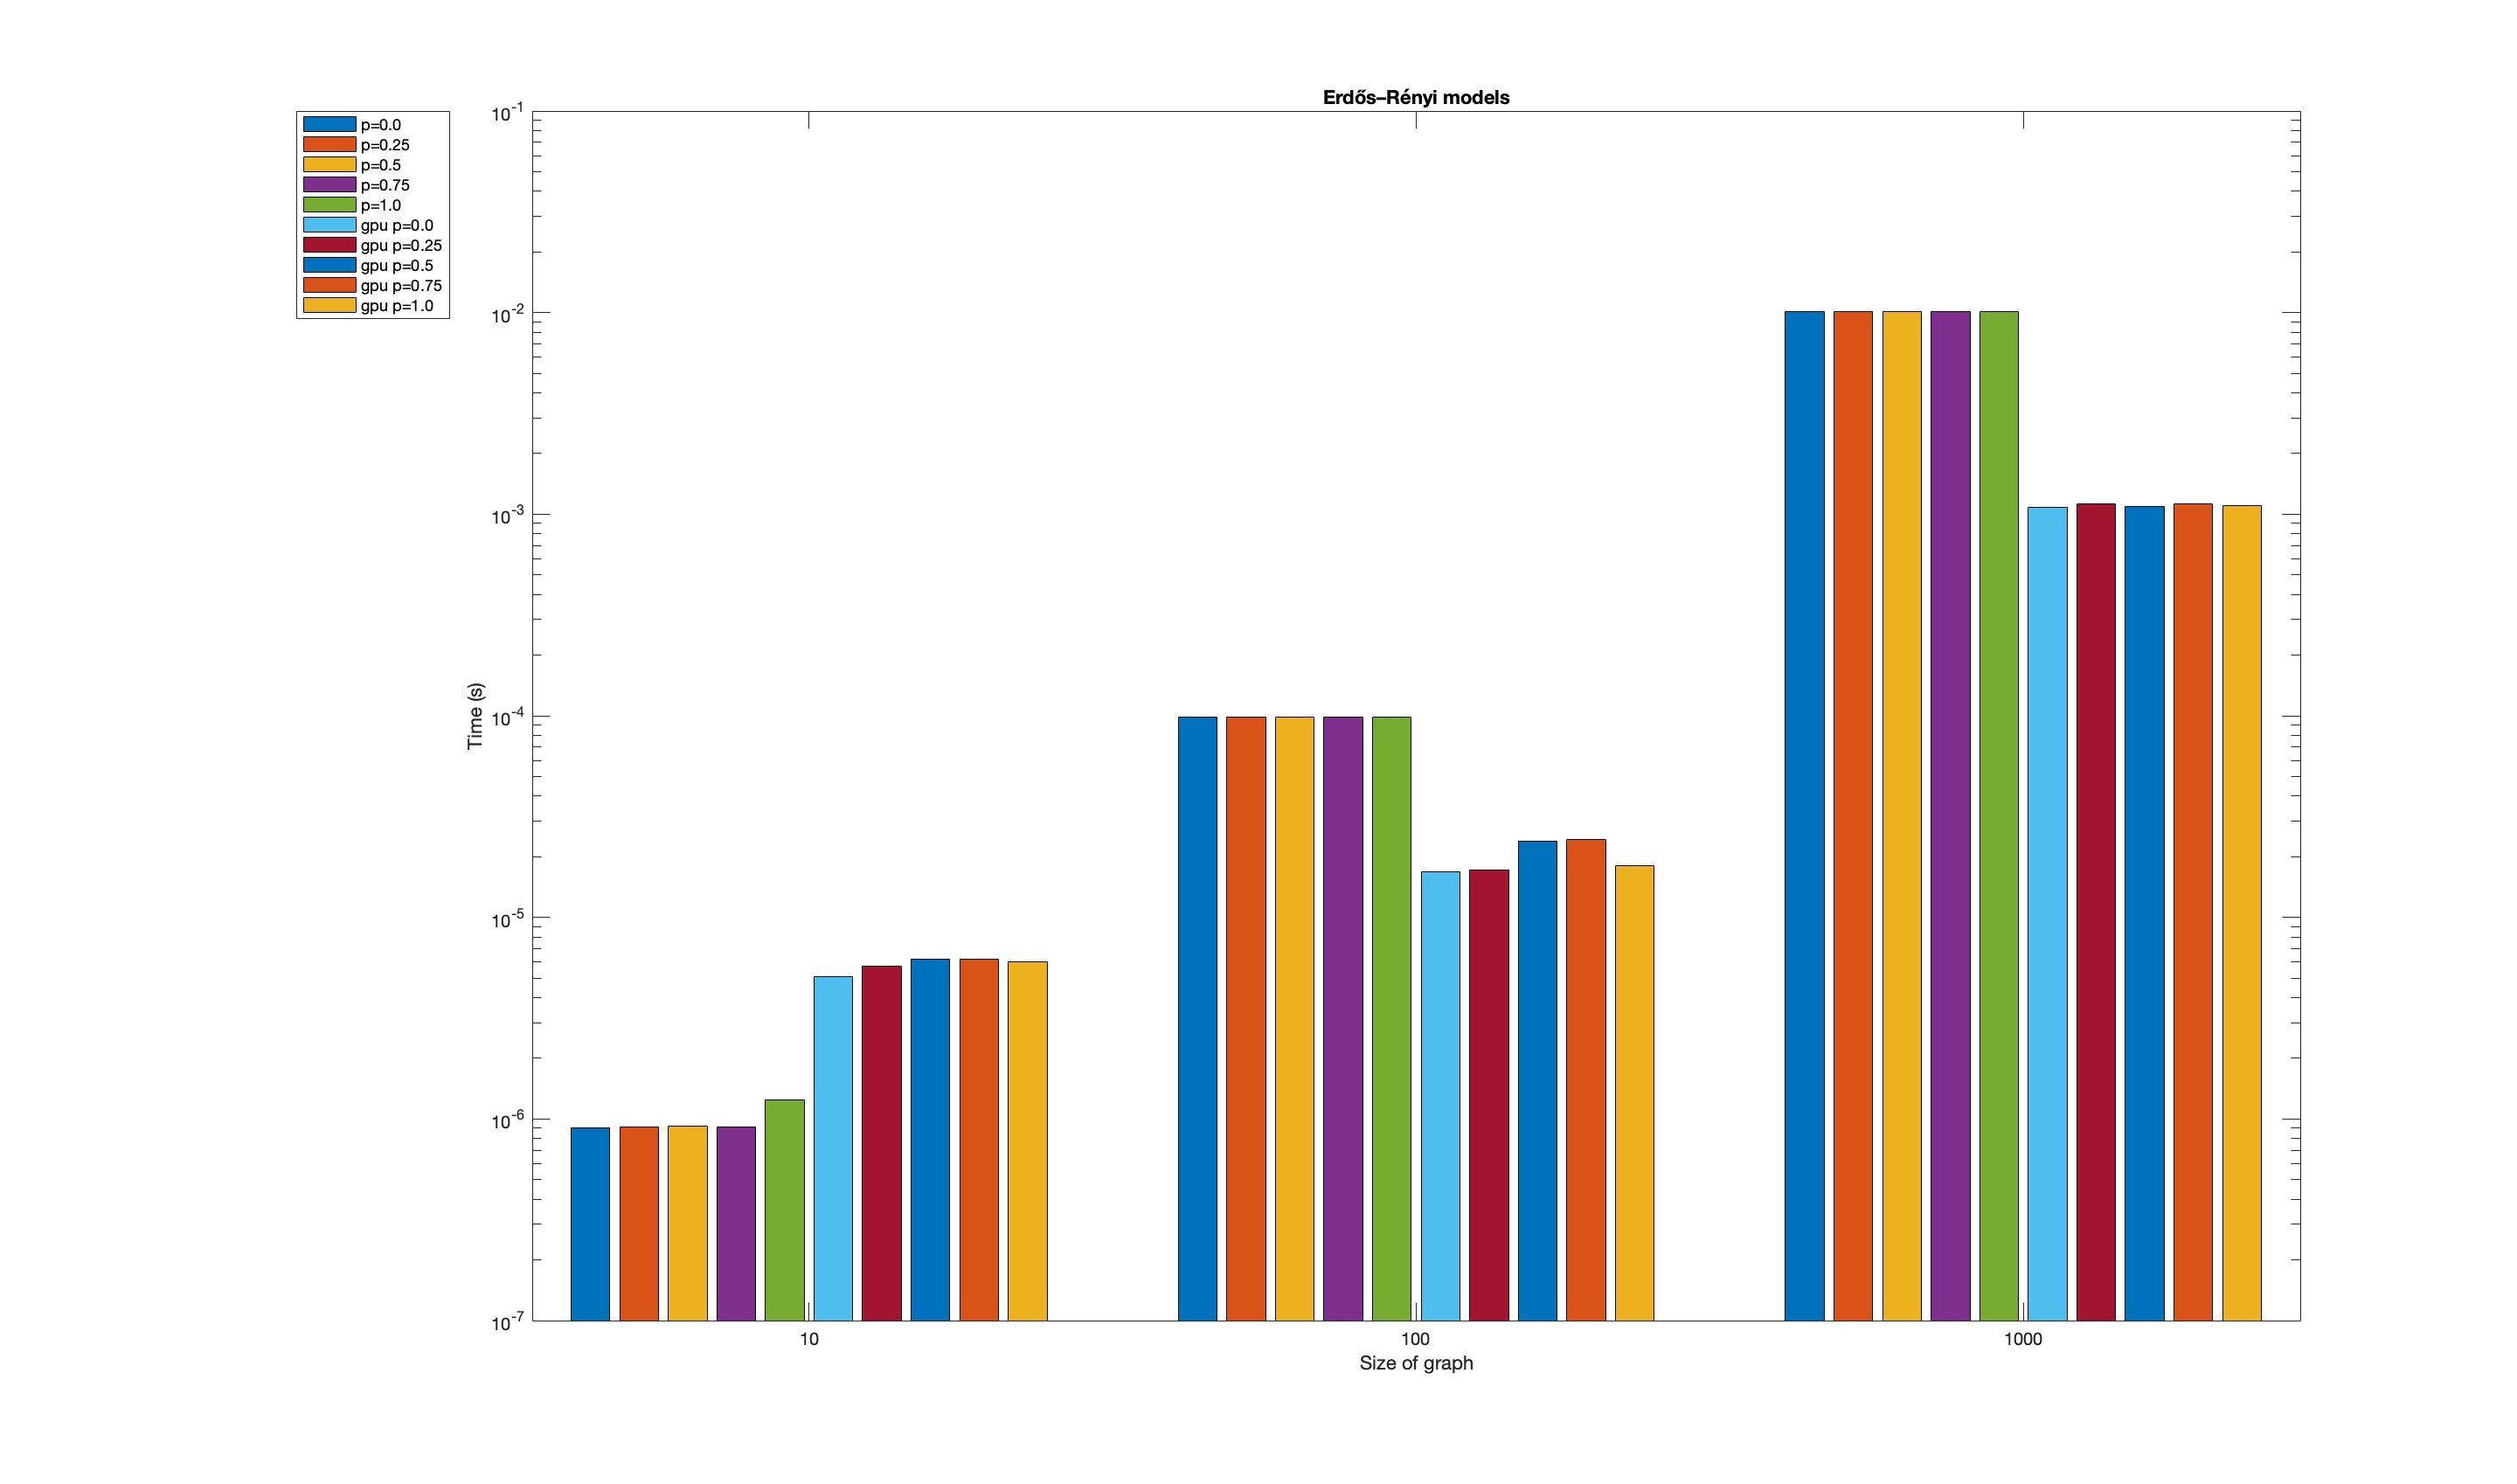
\includegraphics[width=\textwidth]{img/ER.jpg}
    \caption{Times for generation of a random graph with the ER model}
    \label{fig:ER}
\end{figure}

\begin{table}[H]
\makebox[\linewidth]{
\begin{tabular}{|c|c|c|c|c|c|c|c|}
 \hline
 \multirow{2}{*}{k} & \multirow{2}{*}{Type} & \multicolumn{5}{|c|}{Mean WS random graph generation times for size 10 (s)} \\
 \cline{3-7}
 & & p=0.0 & p=0.25 & p=0.5 & p=0.75 & p=1.0\\
 \hline
 \hline
 \multirow{2}{*}{2} & Sequential & 2.3599e-07 & 2.7200e-07 & 2.5800e-07 & 2.9400e-07 & 3.3200e-07 \\
 \cline{2-7}
 & Parallel & 5.8250e-06 & 5.1080e-06 & 6.0549e-06 & 5.9129e-06 & 5.1710e-06 \\
 \hline
 \hline
 \multirow{2}{*}{4} & Sequential & 2.7399e-07 & 3.6900e-07 & 4.2099e-07 & 4.8599e-07 & 4.9299e-07 \\
 \cline{2-7}
 & Parallel & 5.2909e-06 & 5.3970e-06 & 6.4969e-06 & 6.2769e-06 & 5.4079e-06 \\
 \hline
 \hline
 \multirow{2}{*}{6} & Sequential & 3.9700e-07 & 5.0900e-07 & 6.3100e-07 & 6.3100e-07 & 8.4500e-07 \\
 \cline{2-7}
 & Parallel & 5.6150e-06 & 6.3270e-06 & 6.6980e-06 & 5.9599e-06 & 1.1776e-05 \\
 \hline
\end{tabular}
}
\caption{Times of random graph generation of size 10 for the WS algorithm}
\label{tab:WS10}
\end{table}

\begin{figure}[H]
    \centering
    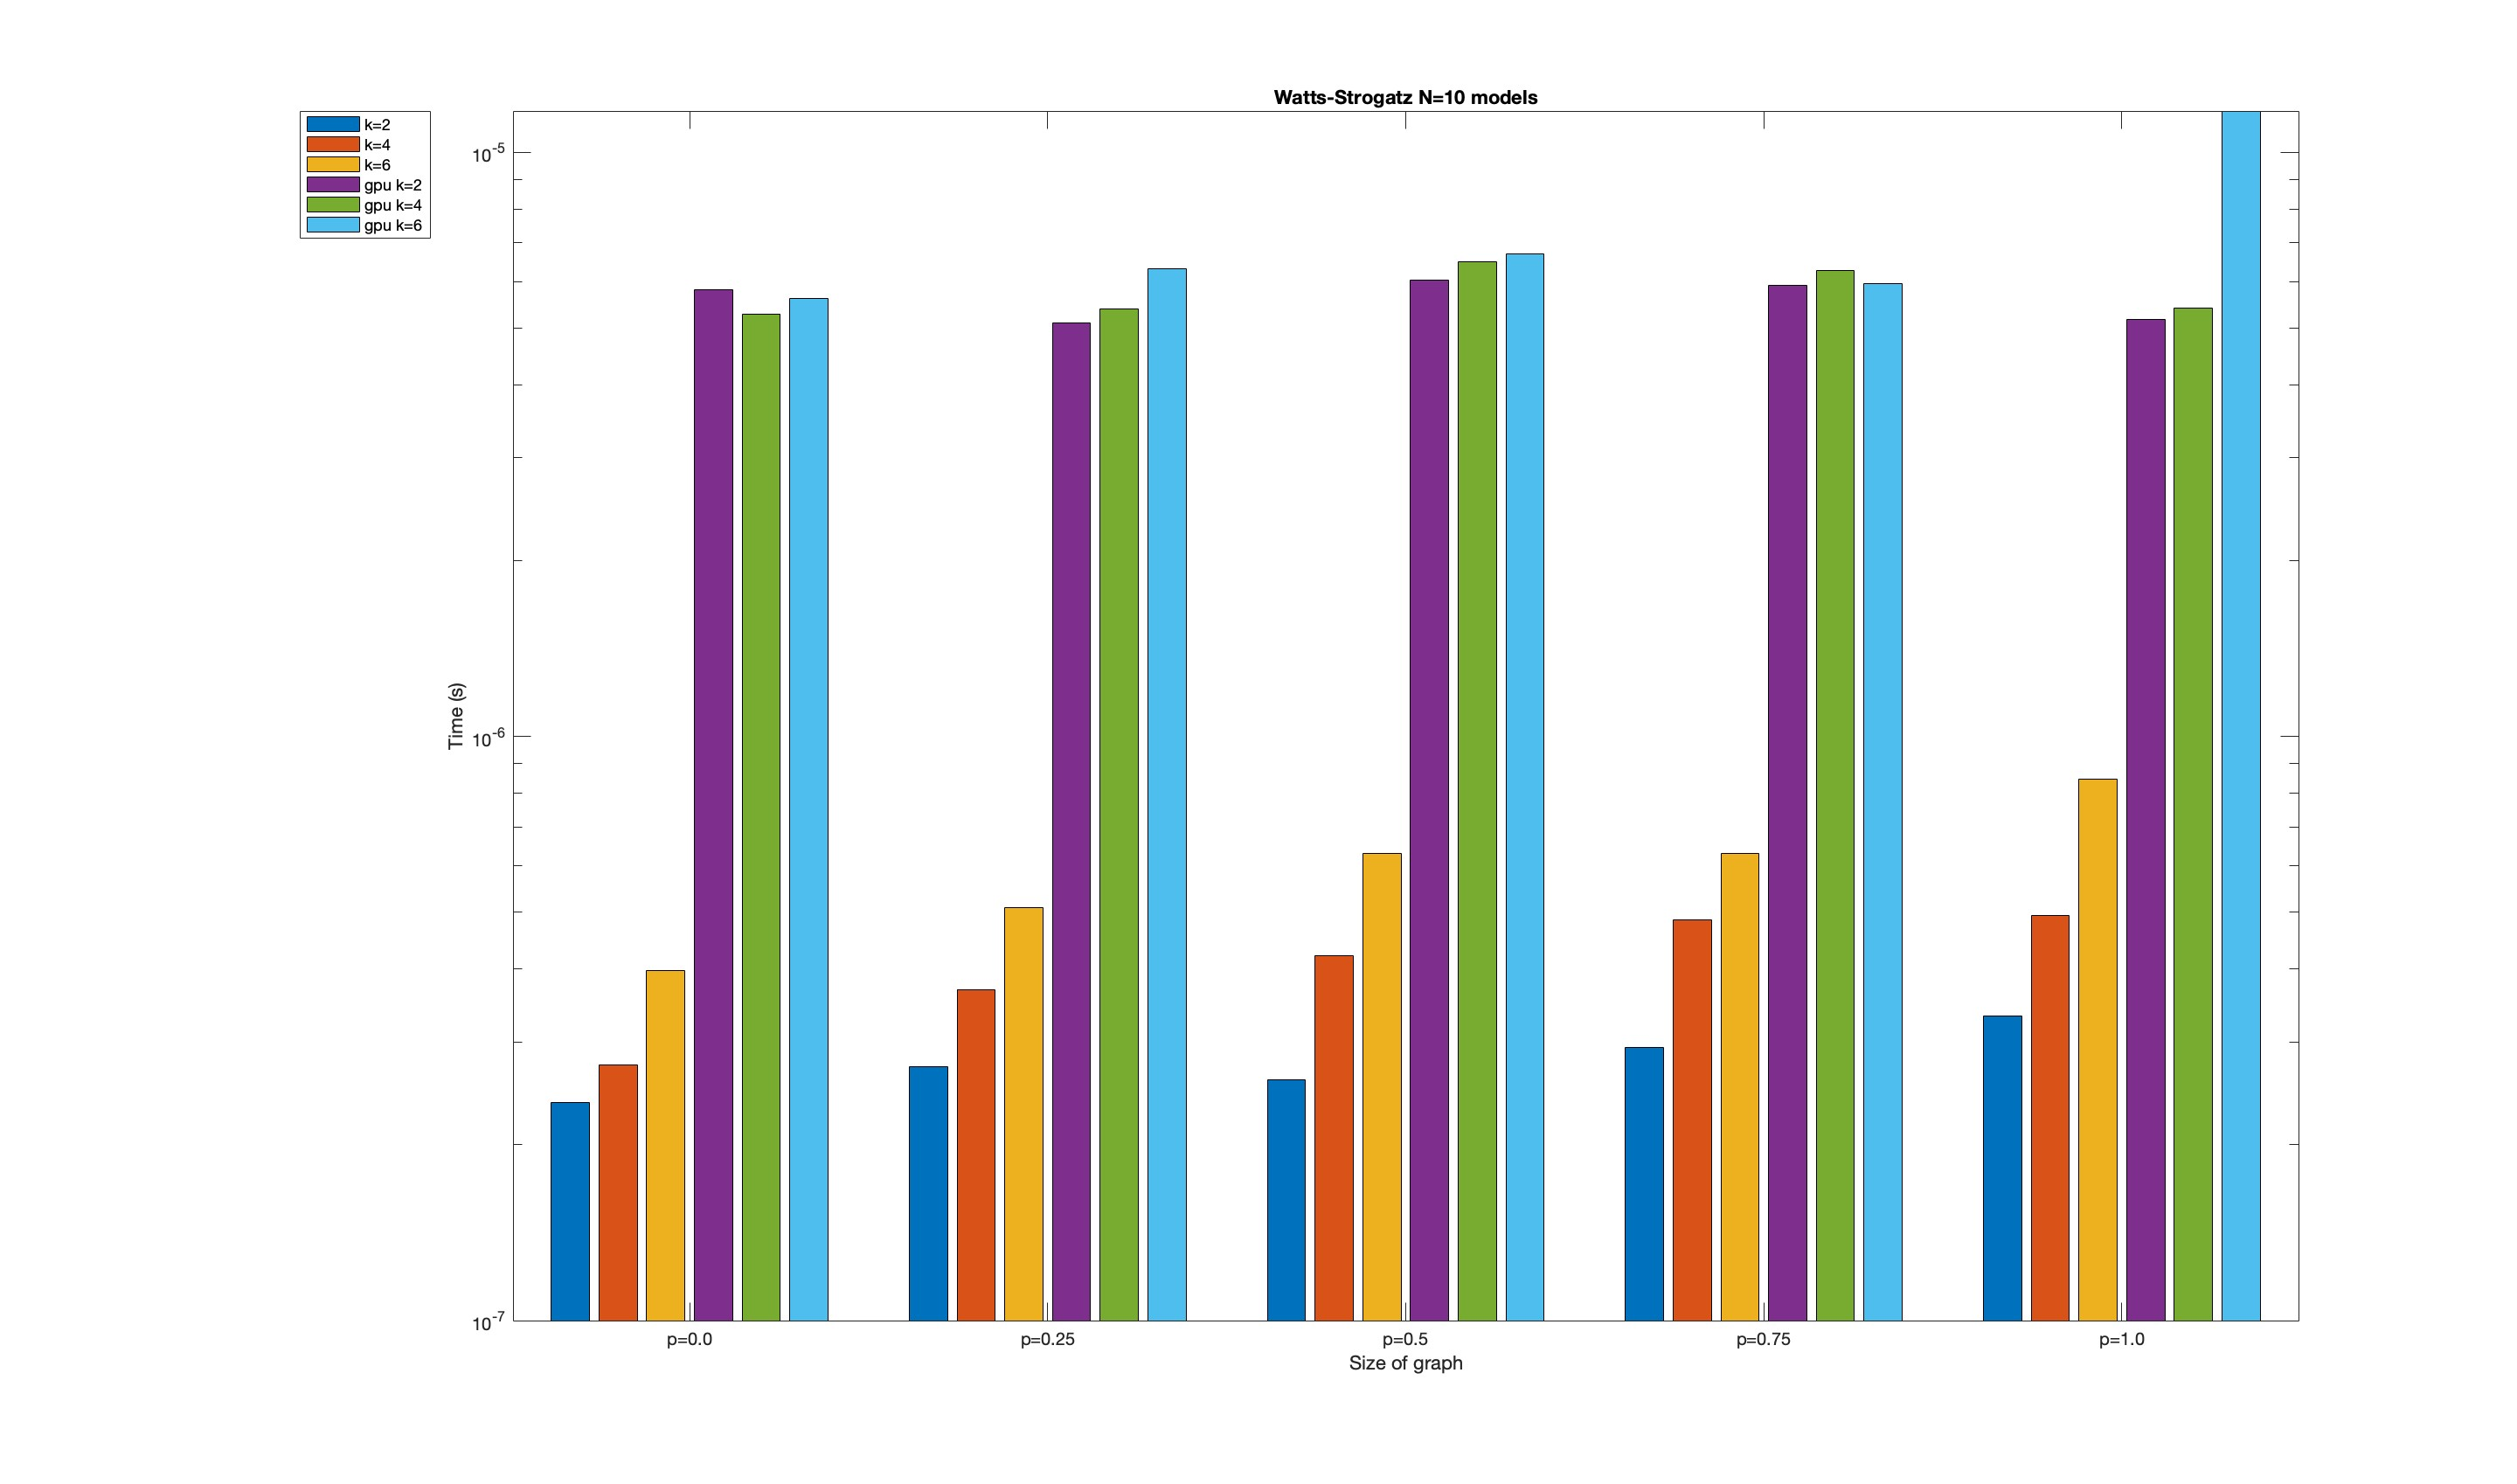
\includegraphics[width=\textwidth]{img/WS10.jpg}
    \caption{Times for generation of a random graph with the WS model (graph size = 10)}
    \label{fig:WS10}
\end{figure}

\begin{table}[H]
\makebox[\linewidth]{
\begin{tabular}{|c|c|c|c|c|c|c|c|}
 \hline
 \multirow{2}{*}{k} & \multirow{2}{*}{Type} & \multicolumn{5}{|c|}{Mean WS random graph generation times for size 100 (s)} \\
 \cline{3-7}
 & & p=0.0 & p=0.25 & p=0.5 & p=0.75 & p=1.0\\
 \hline
 \hline
 \multirow{2}{*}{2} & Sequential & 8.1290e-06 & 1.1407e-05 & 8.0050e-06 & 1.1844e-05 & 1.0751e-05 \\
 \cline{2-7}
 & Parallel & 7.0380e-06 & 5.8659e-06 & 7.4170e-06 & 5.1590e-06 & 5.1819e-06 \\
 \hline
 \hline
 \multirow{2}{*}{4} & Sequential & 7.9710e-06 & 9.1730e-06 & 9.1710e-06 & 1.4361e-05 & 1.2217e-05 \\
 \cline{2-7}
 & Parallel & 5.4060e-06 & 6.5799e-06 & 7.8619e-06 & 5.5099e-06 & 7.5549e-06 \\
 \hline
 \hline
 \multirow{2}{*}{6} & Sequential & 1.5258e-05 & 1.4800e-05 & 1.5965e-05 & 1.6379e-05 & 1.3159e-05 \\
 \cline{2-7}
 & Parallel & 6.3899e-06 & 5.7869e-06 & 9.2949e-06 & 6.3090e-06 & 6.5039e-06 \\
 \hline
\end{tabular}
}
\caption{Times of random graph generation of size 100 for the WS algorithm}
\label{tab:WS100}
\end{table}

\begin{figure}[H]
    \centering
    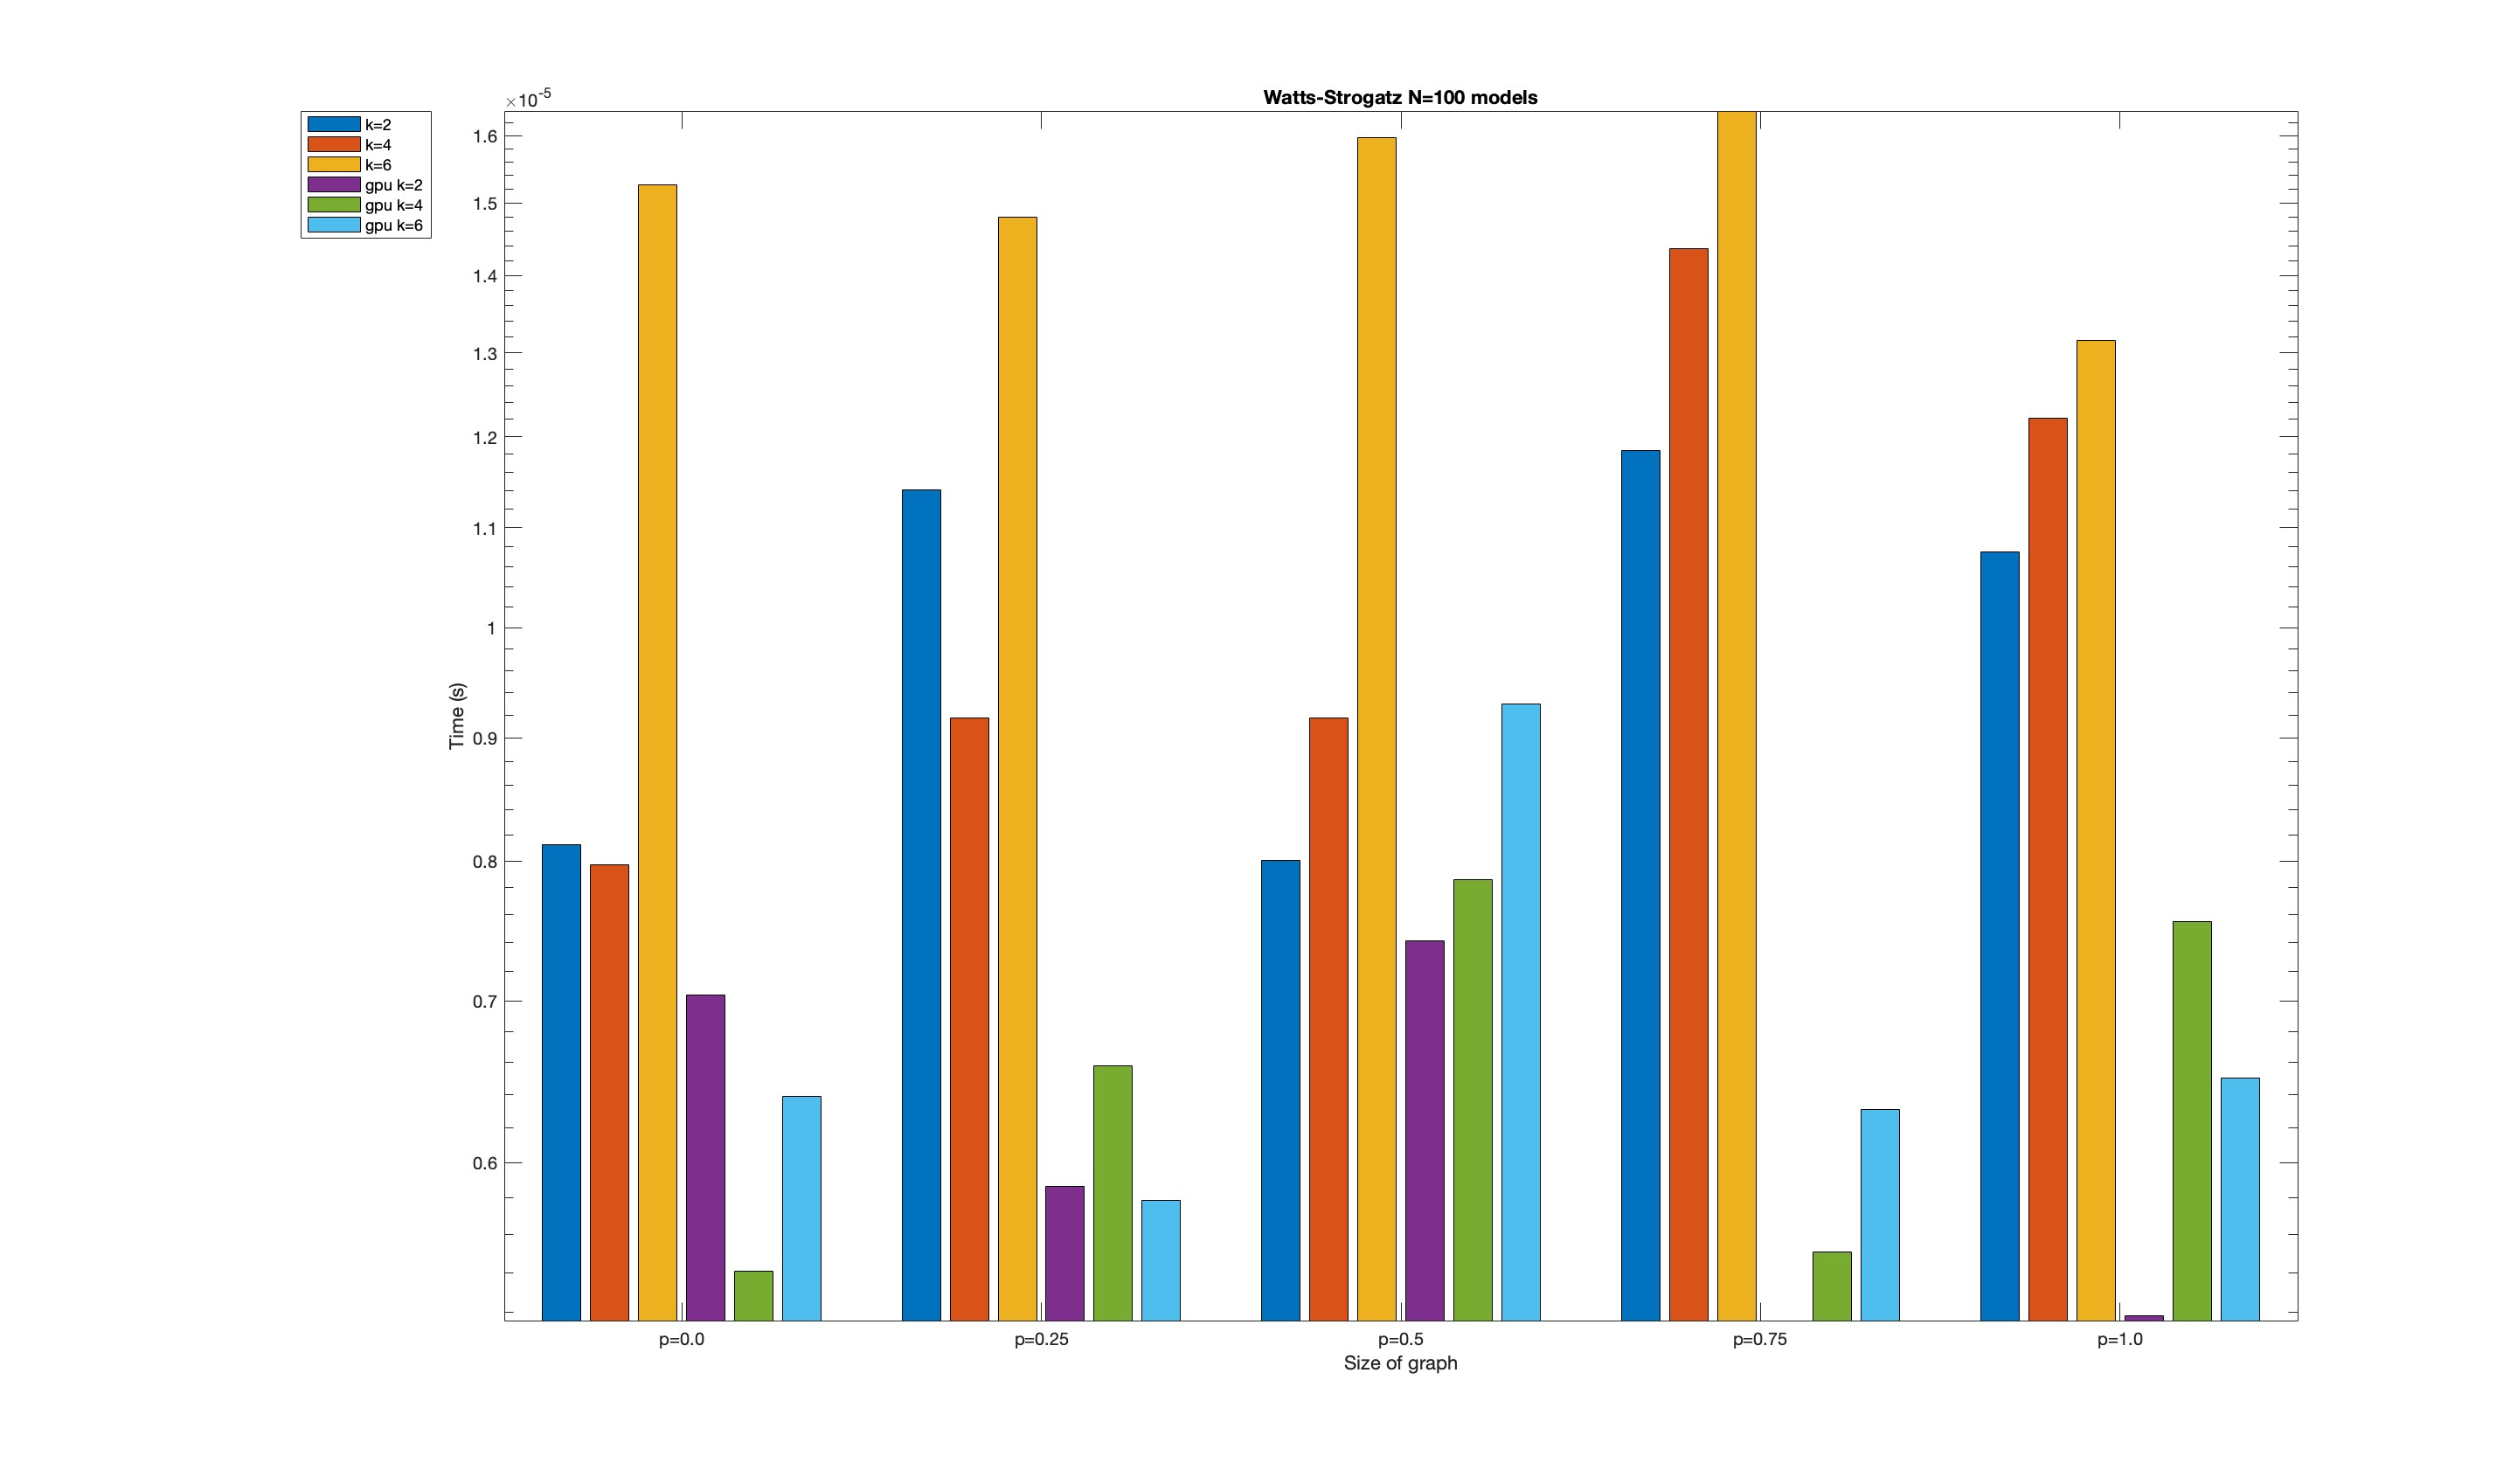
\includegraphics[width=\textwidth]{img/WS100.jpg}
    \caption{Times for generation of a random graph with the WS model (graph size = 100)}
    \label{fig:WS100}
\end{figure}

\begin{table}[H]
\makebox[\linewidth]{
\begin{tabular}{|c|c|c|c|c|c|c|c|}
 \hline
 \multirow{2}{*}{k} & \multirow{2}{*}{Type} & \multicolumn{5}{|c|}{Mean WS random graph generation times for size 1000 (s)} \\
 \cline{3-7}
 & & p=0.0 & p=0.25 & p=0.5 & p=0.75 & p=1.0\\
 \hline
 \hline
 \multirow{2}{*}{2} & Sequential & 8.5567e-04 & 8.6808e-04 & 8.2603e-04 & 8.2840e-04 & 8.7826e-04 \\
 \cline{2-7}
 & Parallel & 7.7850e-06 & 7.2760e-06 & 7.5220e-06 & 8.3159e-06 & 7.9590e-06 \\
 \hline
 \hline
 \multirow{2}{*}{4} & Sequential & 8.4732e-04 & 9.3006e-04 & 8.8170e-04 & 9.3210e-04 & 8.5639e-04 \\
 \cline{2-7}
 & Parallel & 8.2900e-06 & 1.0778e-05 & 9.0240e-06 & 8.8009e-06 & 9.0489e-06 \\
 \hline
 \hline
 \multirow{2}{*}{6} & Sequential & 8.6740e-04 & 1.0109e-03 & 8.4060e-04 & 8.6691e-04 & 9.5498e-04 \\
 \cline{2-7}
 & Parallel & 8.6189e-06 & 8.5099e-06 & 9.8530e-06 & 1.2326e-05 & 1.3004e-05 \\
 \hline
\end{tabular}
}
\caption{Times of random graph generation of size 1000 for the WS algorithm}
\label{tab:WS1000}
\end{table}

\begin{figure}[H]
    \centering
    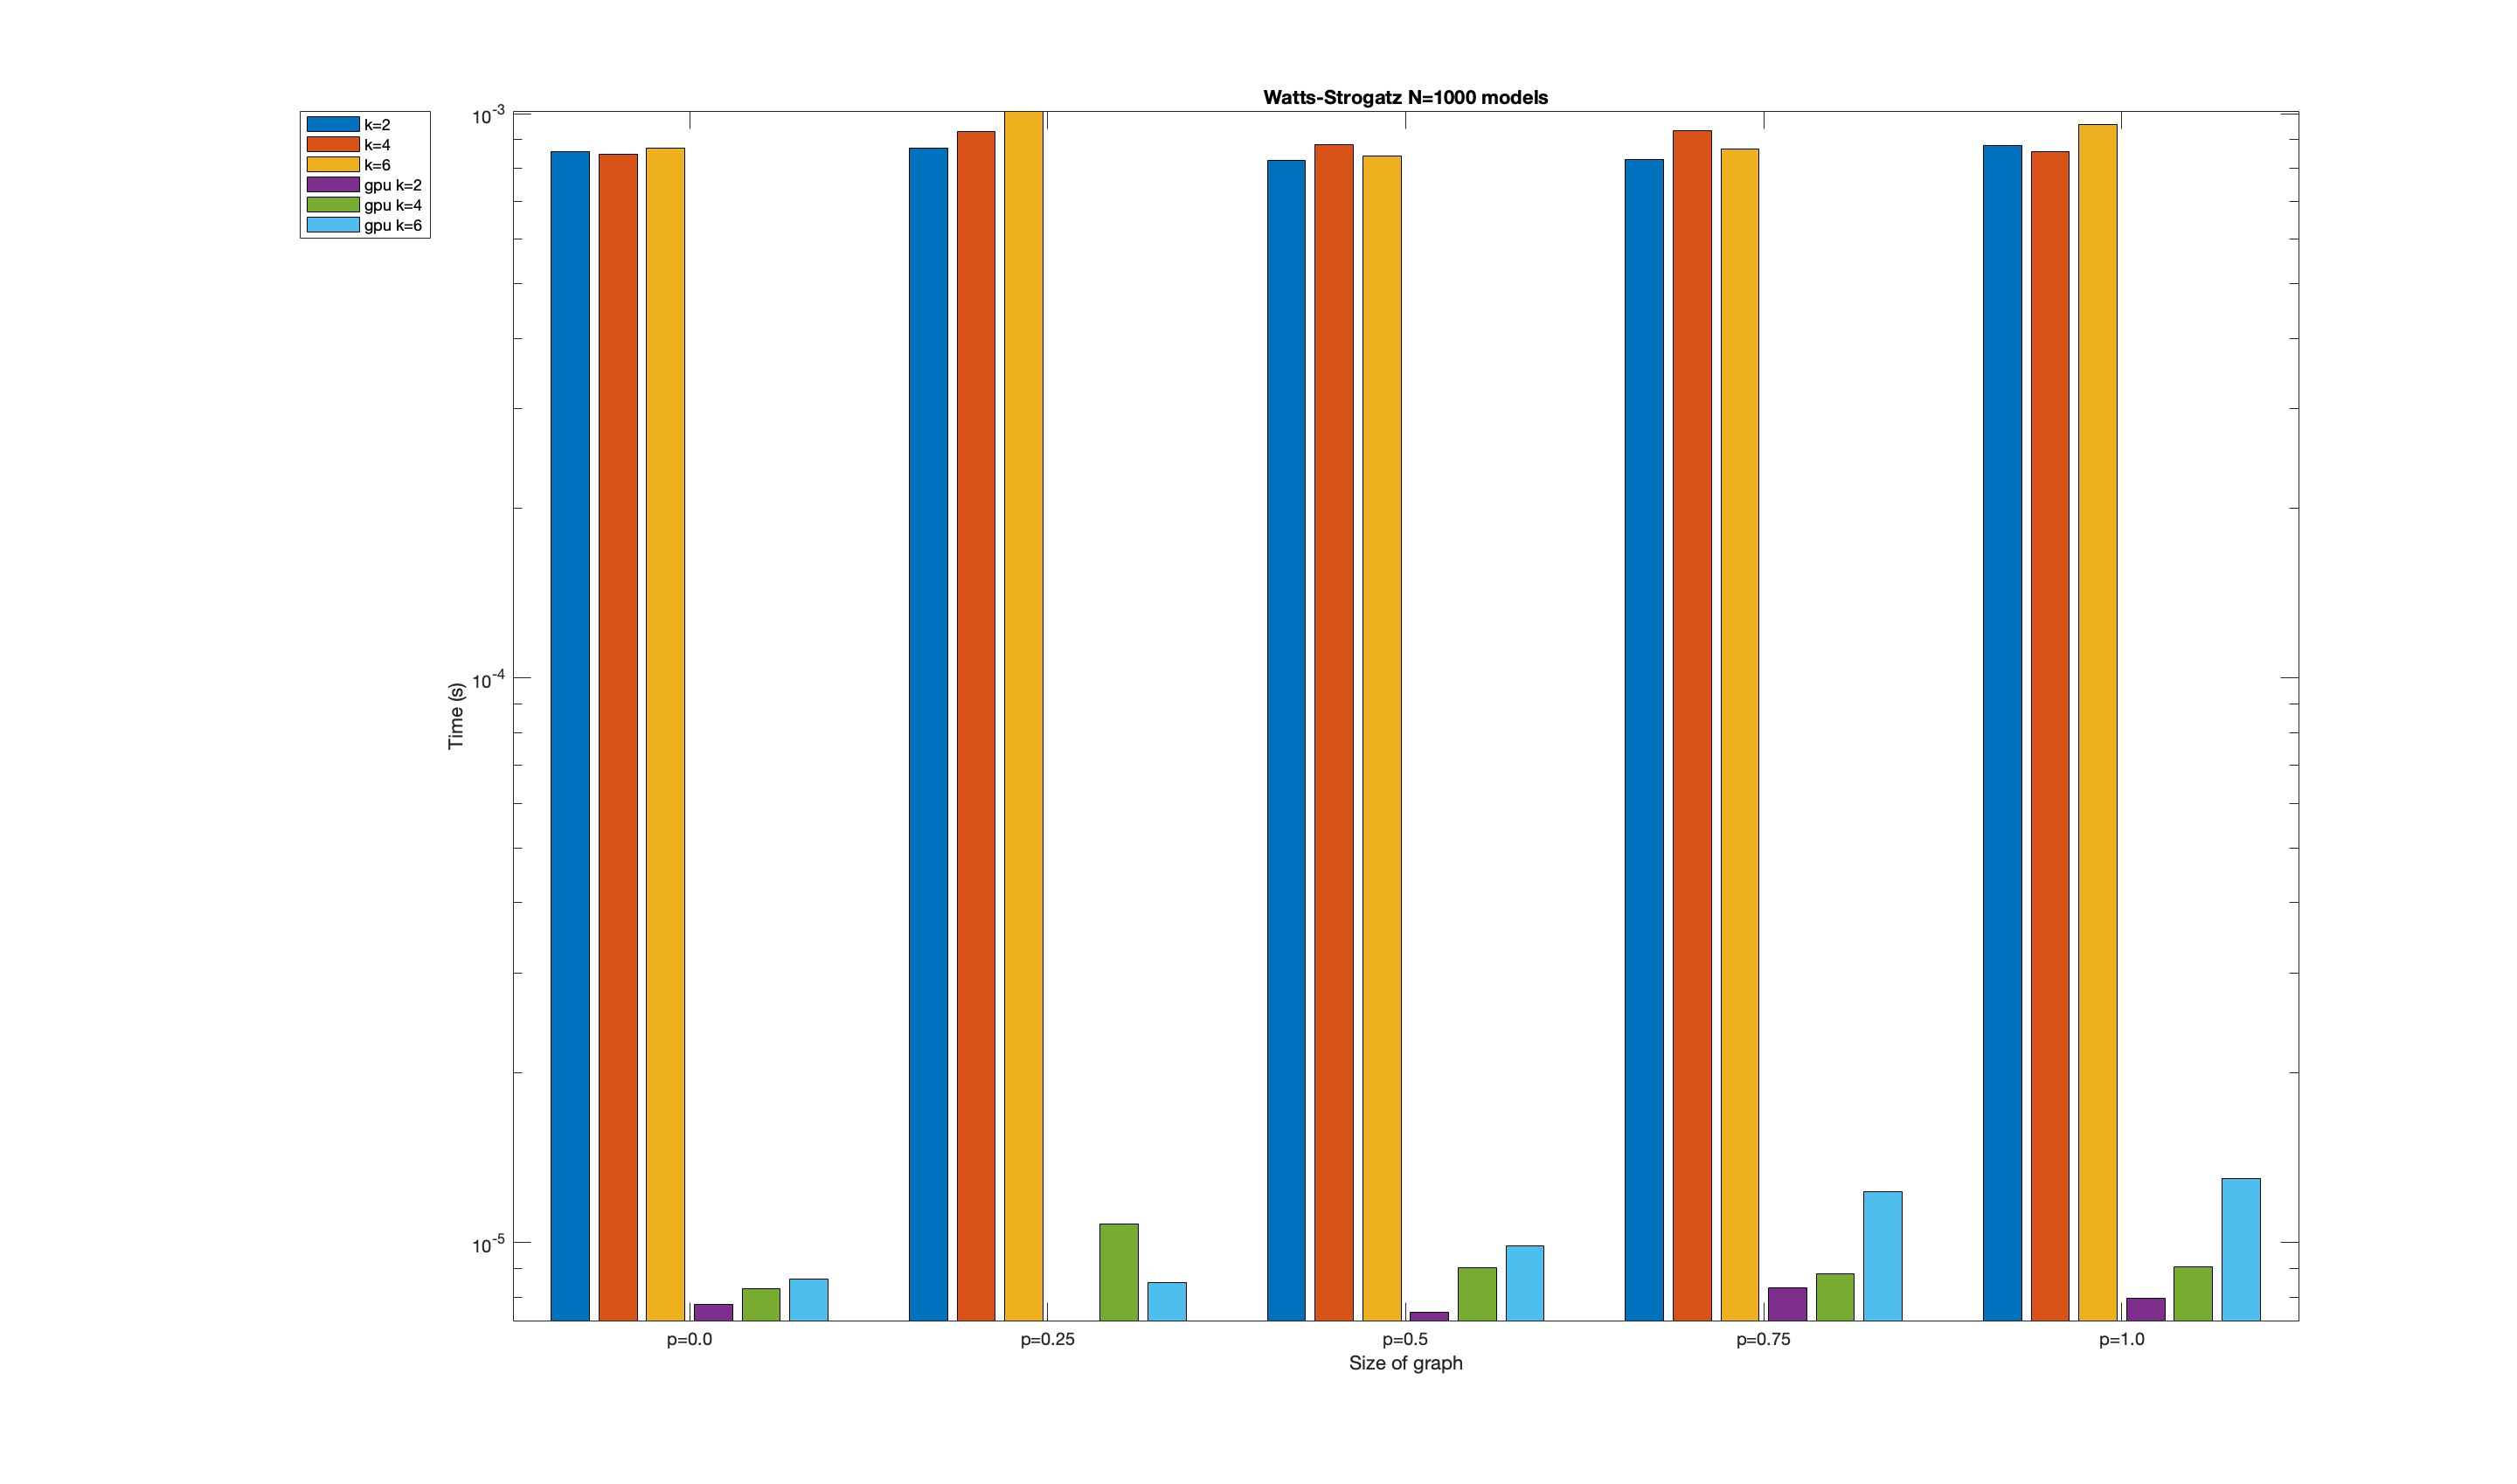
\includegraphics[width=\textwidth]{img/WS1000.jpg}
    \caption{Times for generation of a random graph with the WS model (graph size = 1000)}
    \label{fig:WS1000}
\end{figure}

\begin{table}[H]
\makebox[\linewidth]{
\begin{tabular}{|c|c|c|c|c|c|c|c|}
 \hline
 \multirow{2}{*}{Graph size} & \multirow{2}{*}{Type} & \multicolumn{5}{|c|}{Mean RGG random graph generation times (s)} \\
 \cline{3-7}
 & & r=0.0 & r=0.25 & r=0.5 & r=0.75 & r=1.0\\
 \hline
 \hline
 \multirow{2}{*}{10 nodes} & Sequential & 2.6200e-07 & 3.0400e-07 & 3.0600e-07 & 3.3399e-07 & 3.3700e-07 \\
 \cline{2-7}
 & Parallel & 1.4087e-05 & 6.6610e-06 & 5.9139e-06 & 6.6969e-06 & 6.7710e-06 \\
 \hline
 \hline
 \multirow{2}{*}{100 nodes} & Sequential & 1.6940e-05 & 2.4759e-05 & 2.9933e-05 & 2.3700e-05 & 2.2212e-05 \\
 \cline{2-7}
 & Parallel & 2.2761e-05 & 2.1811e-05 & 2.1145e-05 & 2.3099e-05 & 2.2315e-05 \\
 \hline
 \hline
 \multirow{2}{*}{1000 nodes} & Sequential & 1.8851e-03 & 3.7473e-03 & 5.3220e-03 & 3.8771e-03 & 2.4333e-03 \\
 \cline{2-7}
 & Parallel & 1.4671e-03 & 1.5237e-03 & 1.4779e-03 & 1.5075e-03 & 1.4681e-03 \\
 \hline
\end{tabular}
}
\caption{Times of random graph generation for the RGG algorithm}
\label{tab:RGG}
\end{table}

\begin{figure}[H]
    \centering
    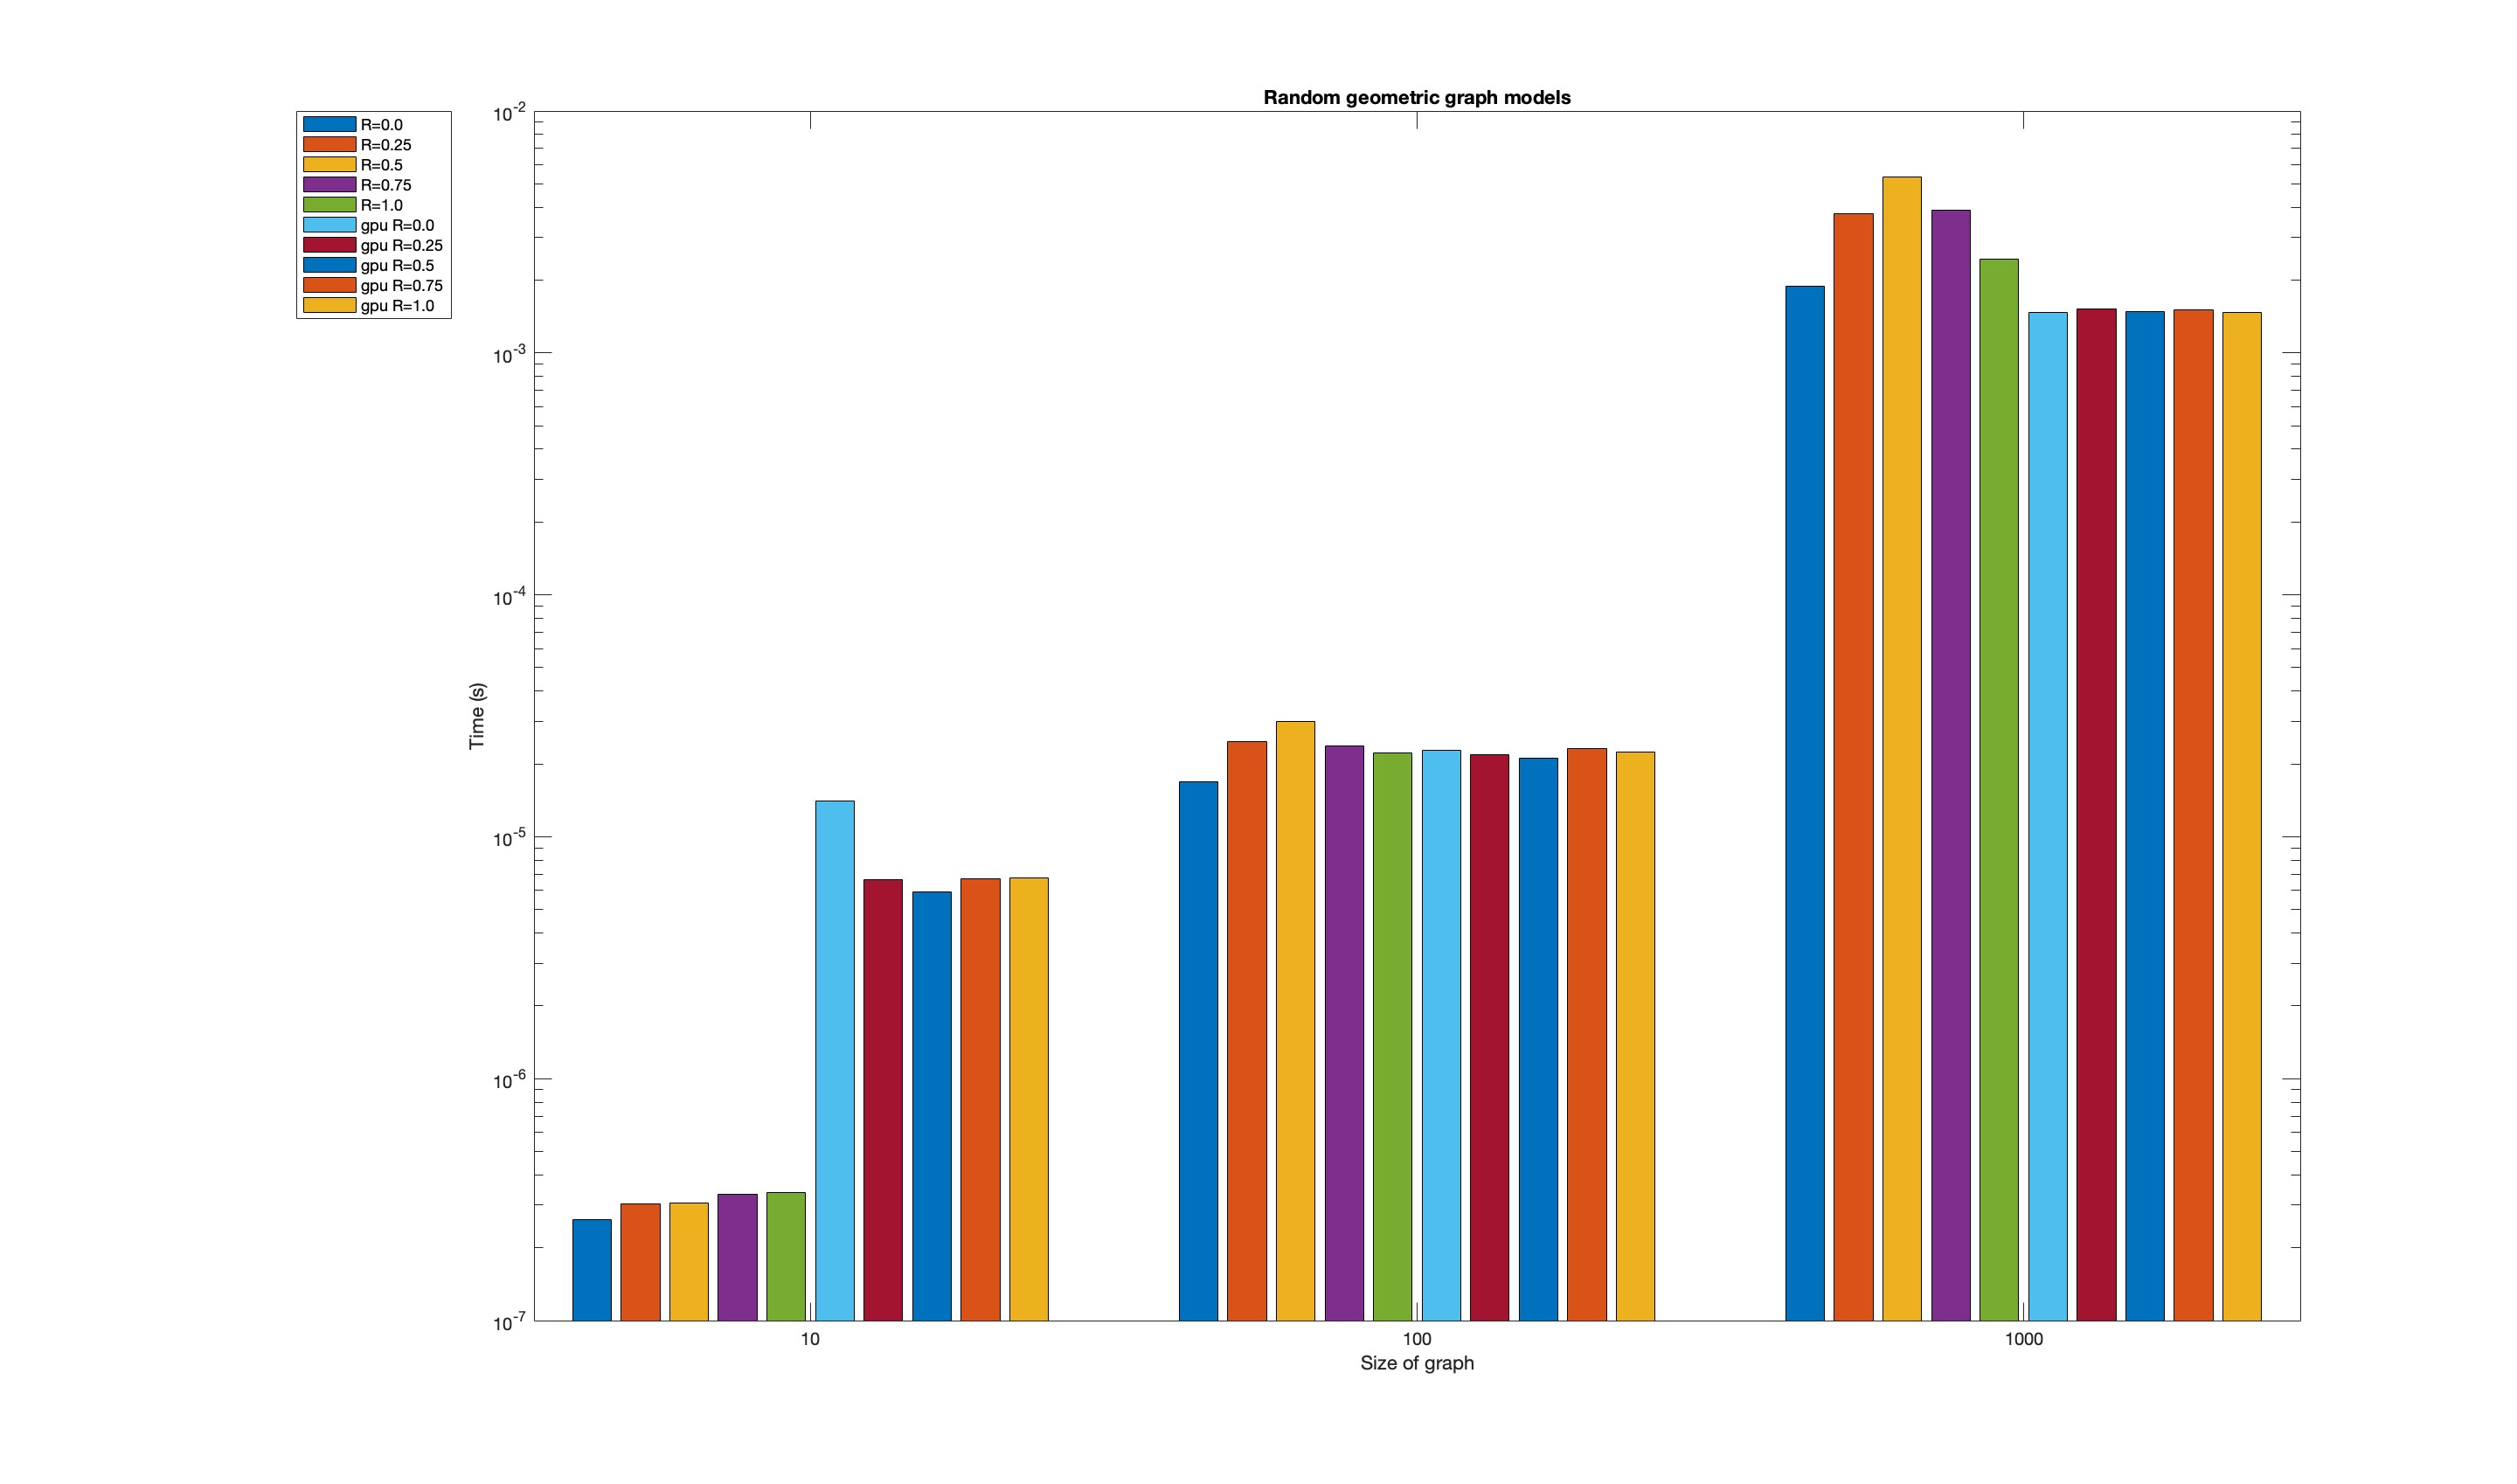
\includegraphics[width=\textwidth]{img/RGG.jpg}
    \caption{Times for generation of a random graph with the RGG model}
    \label{fig:RGG}
\end{figure}

As we can see fropm the results shown above we can make some considerations regarding the parallelization efficiency at lower graph dimensions. In every plot we can see how, for small graphs, the parallel solution is slower than the sequential one; this is probably due to the slower memory access on the gpu as compared to the cpu. Then, considering this difference in memory speed, the parallelization can't give us a speed-up greater than $1$, but in the worst case we presented (RGG for 10 nodes and $r=0.0$) it reaches the value of $0.018598708028678926$.

Yet, we can also see that as the graph size grows, the parallel solution becomes faster than the sequential one, givinge us, in opur best case (WS for 1000 nodes, $k=2$ and $p=0.25$), a speed-up equal to $119.30827377680043$. However we can see that not all parallel solutions are equally as good. Especially in the RGG algorithm case we can see that the advantage of parallelization is almost negligible.

\section{Final thoughts}
Regarding the idea of parallelization for random graph algorithms, we can infer that it is not a convenient practice: most of the time when implementing an algorithm for the generation of a ranodm graph we are interested in models with peculiar characteristics, that are very computationally heavy to implement, and that most of the time, like in the Barabási-Albert model we saw, they depend on their own previous state, making the process of task or even data parallelization very challenging. Of course in this work we merely scratched the tip of the iceberg, focusing just on OpenCL, without exploring other solutions like CUDA or a possible distributed solution, so we have just a narrow vision of the whole problem.

As a future devolpment for this kind of study might be interesting to compare both different parallel OpenCL solutions and solutions obtained with different tools.

\end{document}
